\subsection{Extracción de los procesos con DISCO}

\begin{enumerate}
\item
\item
\item
\end{enumerate}

\begin{figure}[H]
    \centering
    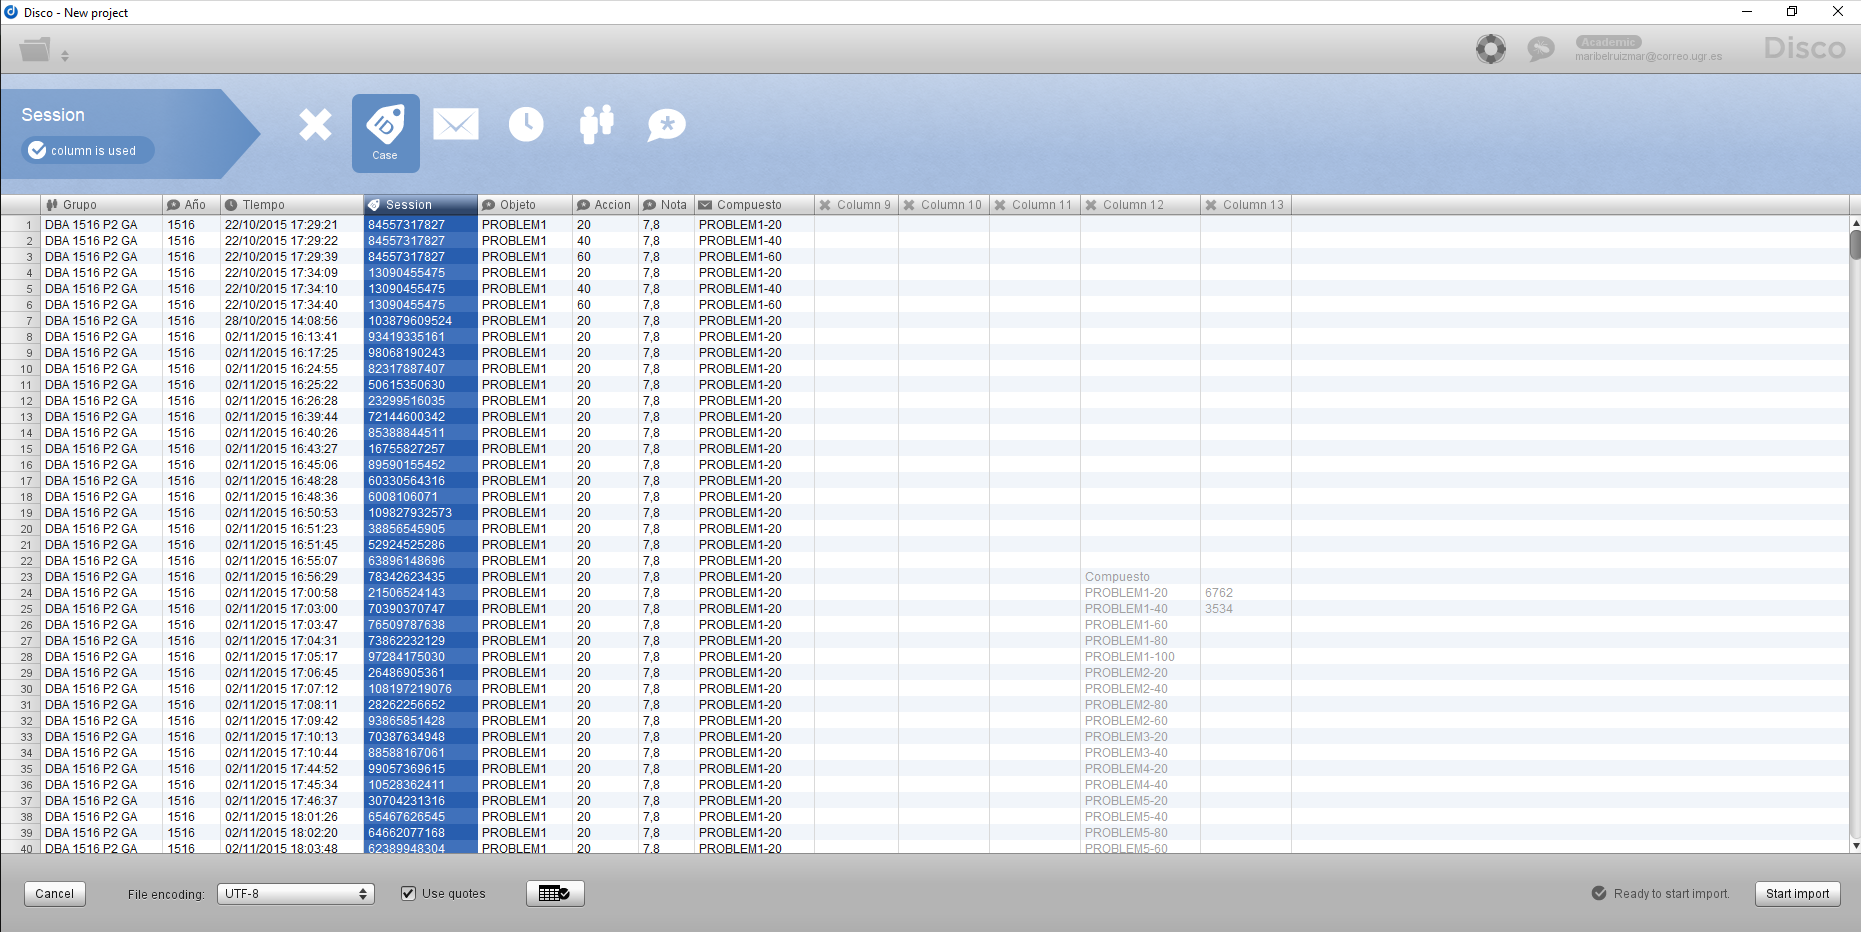
\includegraphics[width=1.25\textwidth]{imagenes/DISCO.png}
    \caption{Análisis de procesos del dataset compuesto.}
    \label{fig:DISCO}
\end{figure}

\begin{figure}[H]
    \centering
    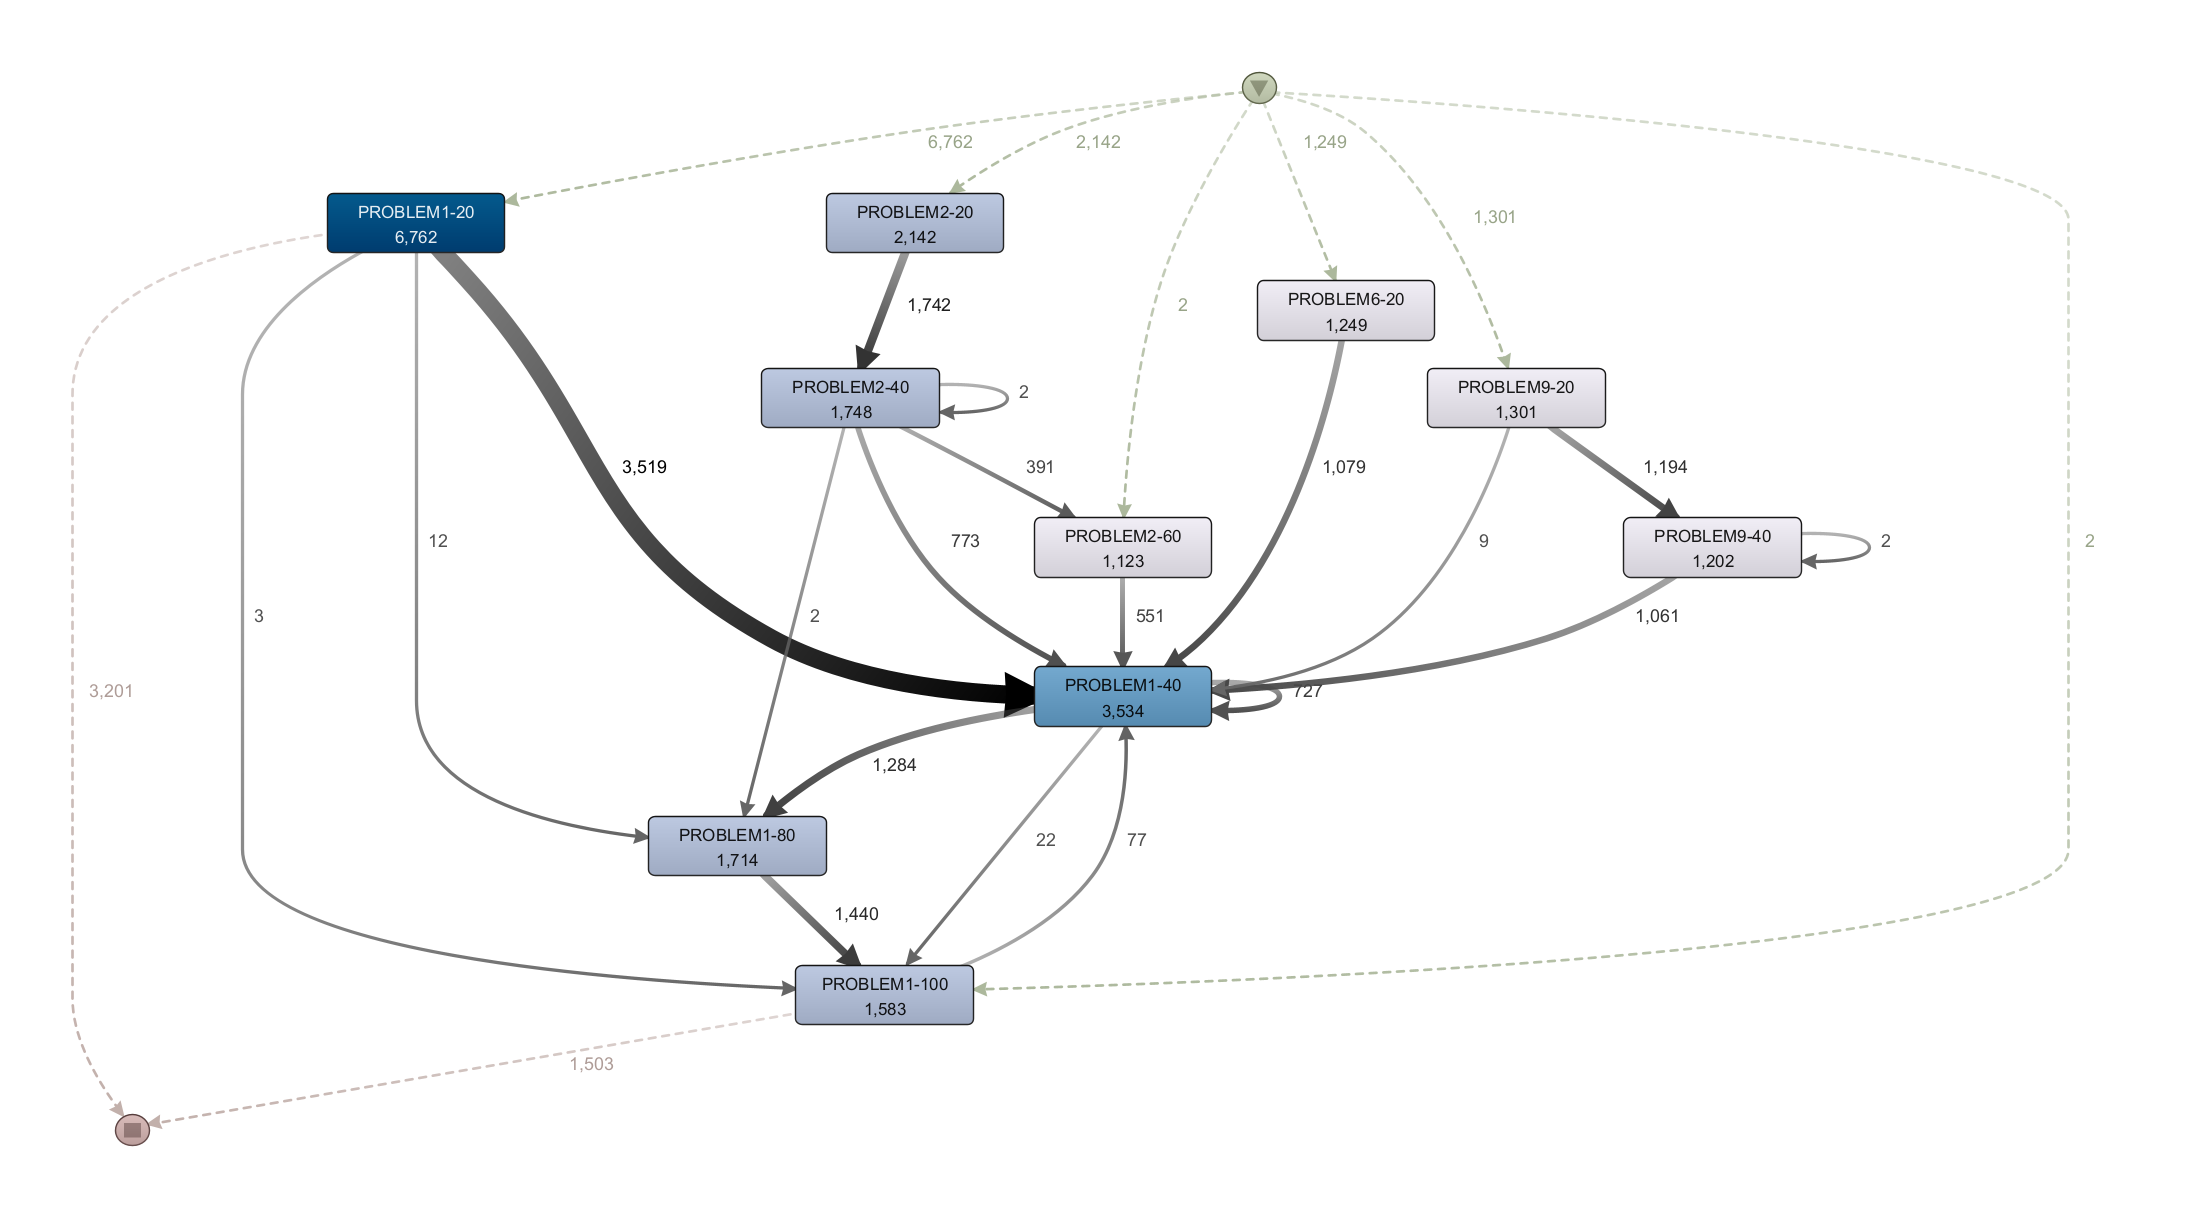
\includegraphics[width=1.25\textwidth]{imagenes/Dataset Fusionado - Compuesto.png}
    \caption{Análisis de procesos del dataset compuesto.}
    \label{fig:datasetFusionado}
\end{figure}

\subsection{Segmentación por años}

\begin{figure}[H]
    \centering
    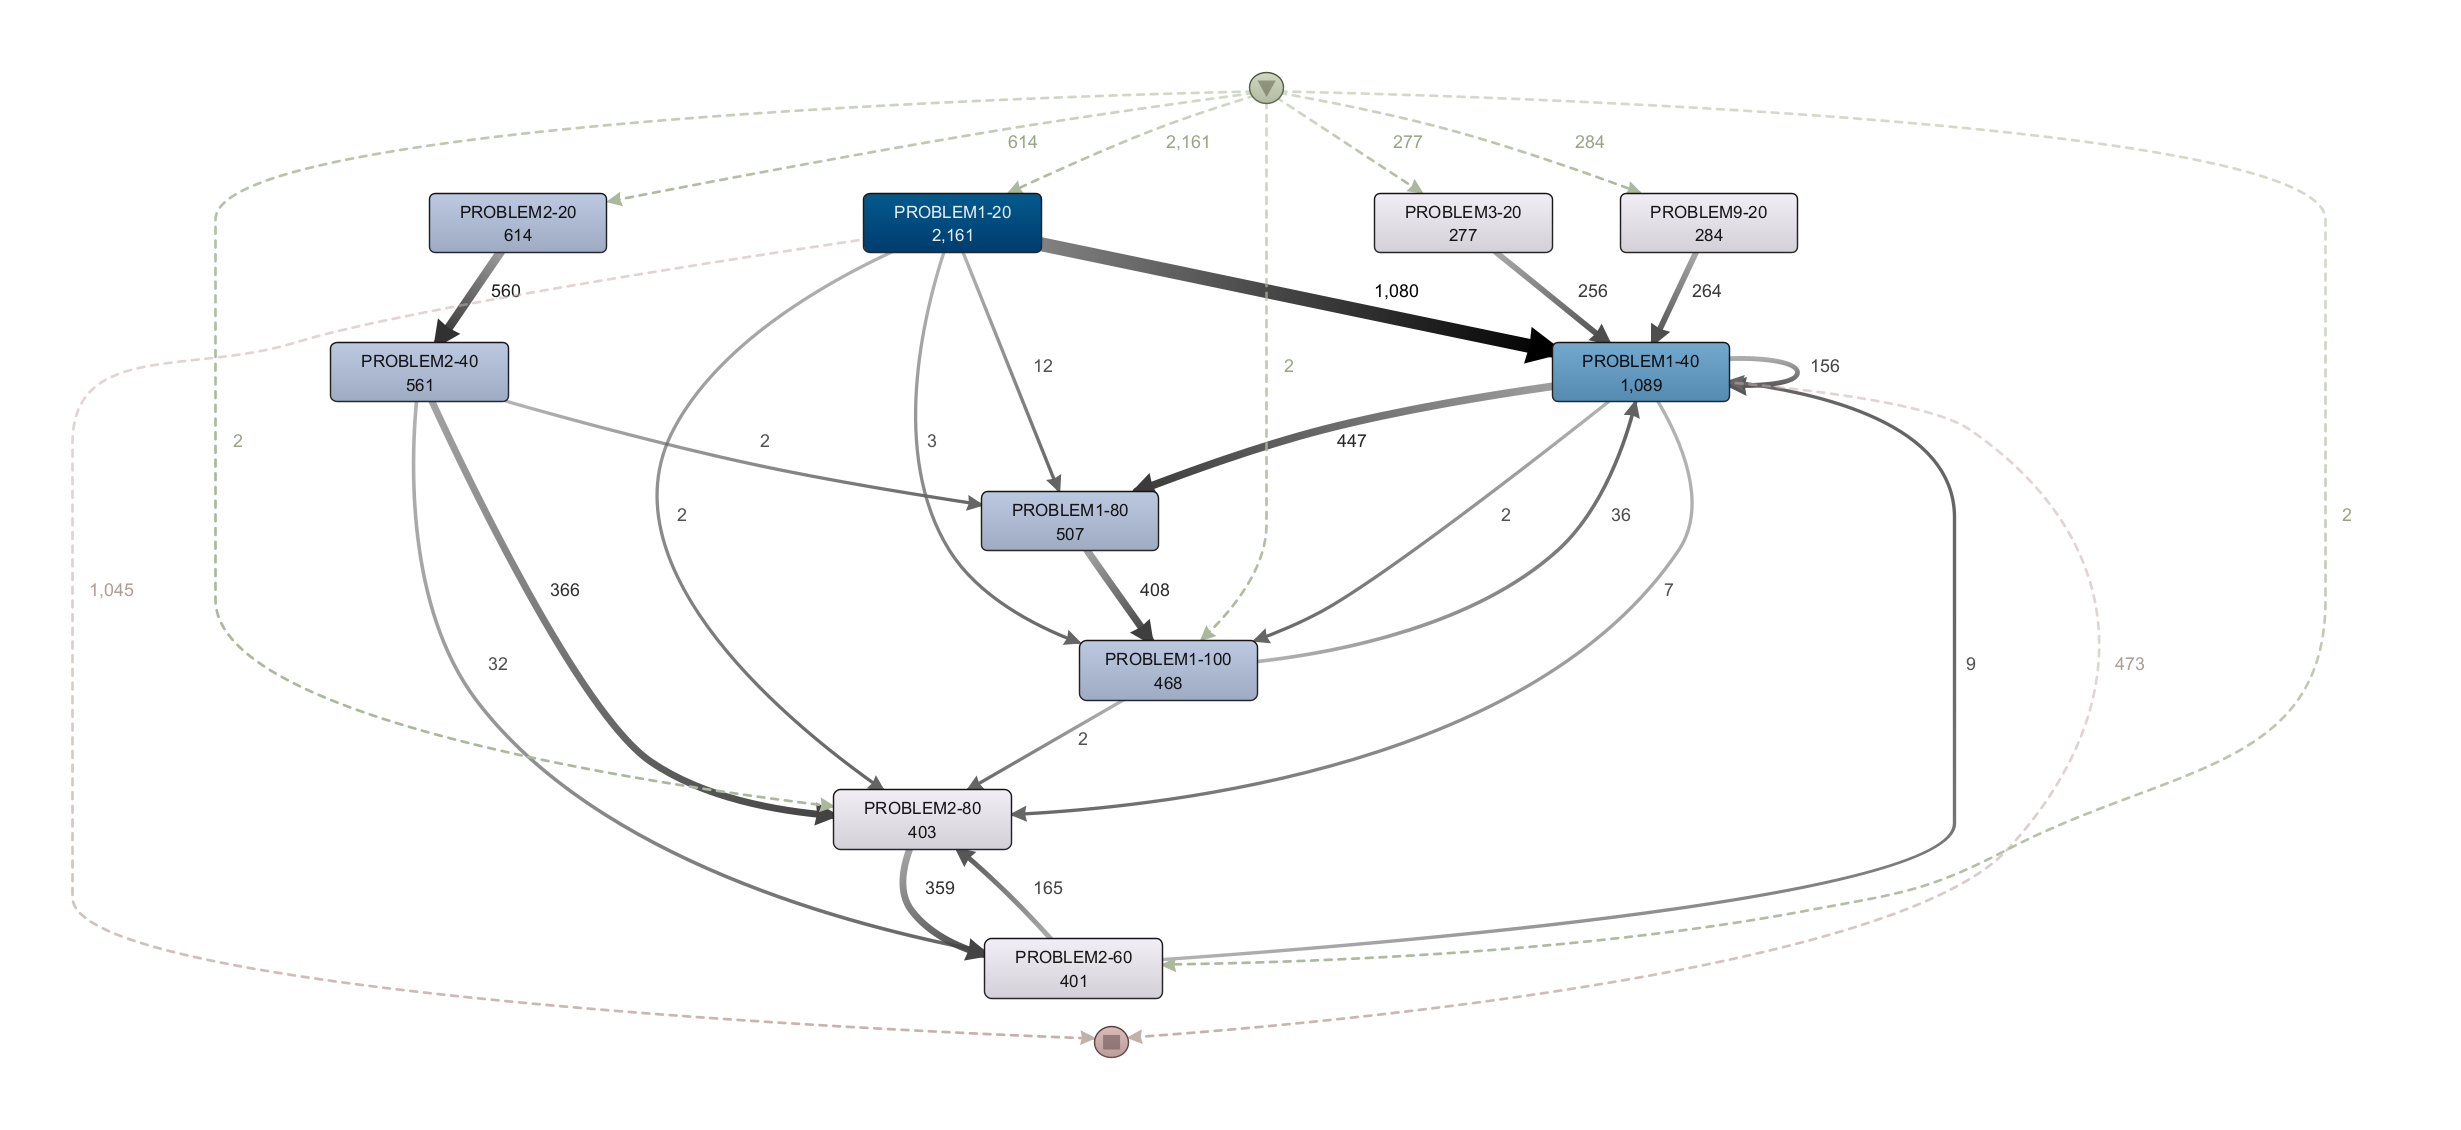
\includegraphics[width=1.25\textwidth]{imagenes/Year1516.png}
    \caption{Extracción de procesos del curso académico 1516.}
    \label{fig:año1516}
\end{figure}

\begin{figure}[H]
    \centering
    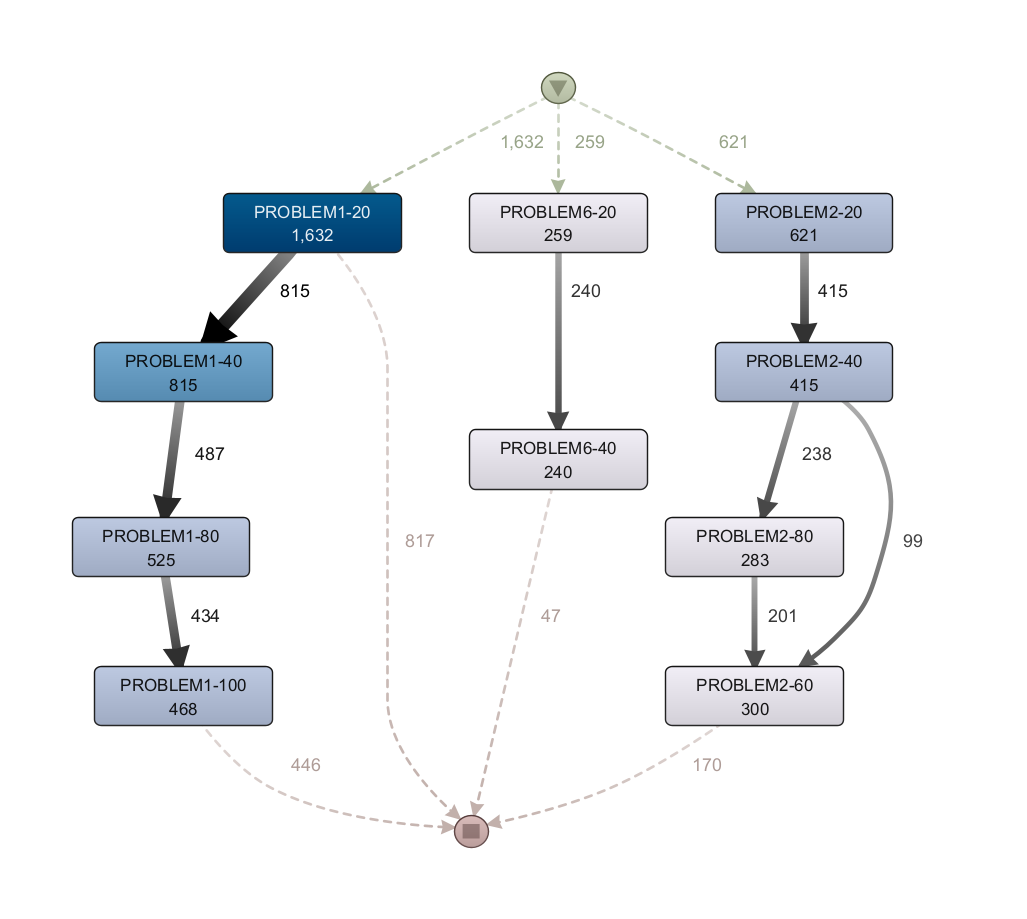
\includegraphics[width=1.25\textwidth]{imagenes/Year1617.png}
    \caption{Extracción de procesos del curso académico 1617.}
    \label{fig:año1617}
\end{figure}

\begin{figure}[H]
    \centering
    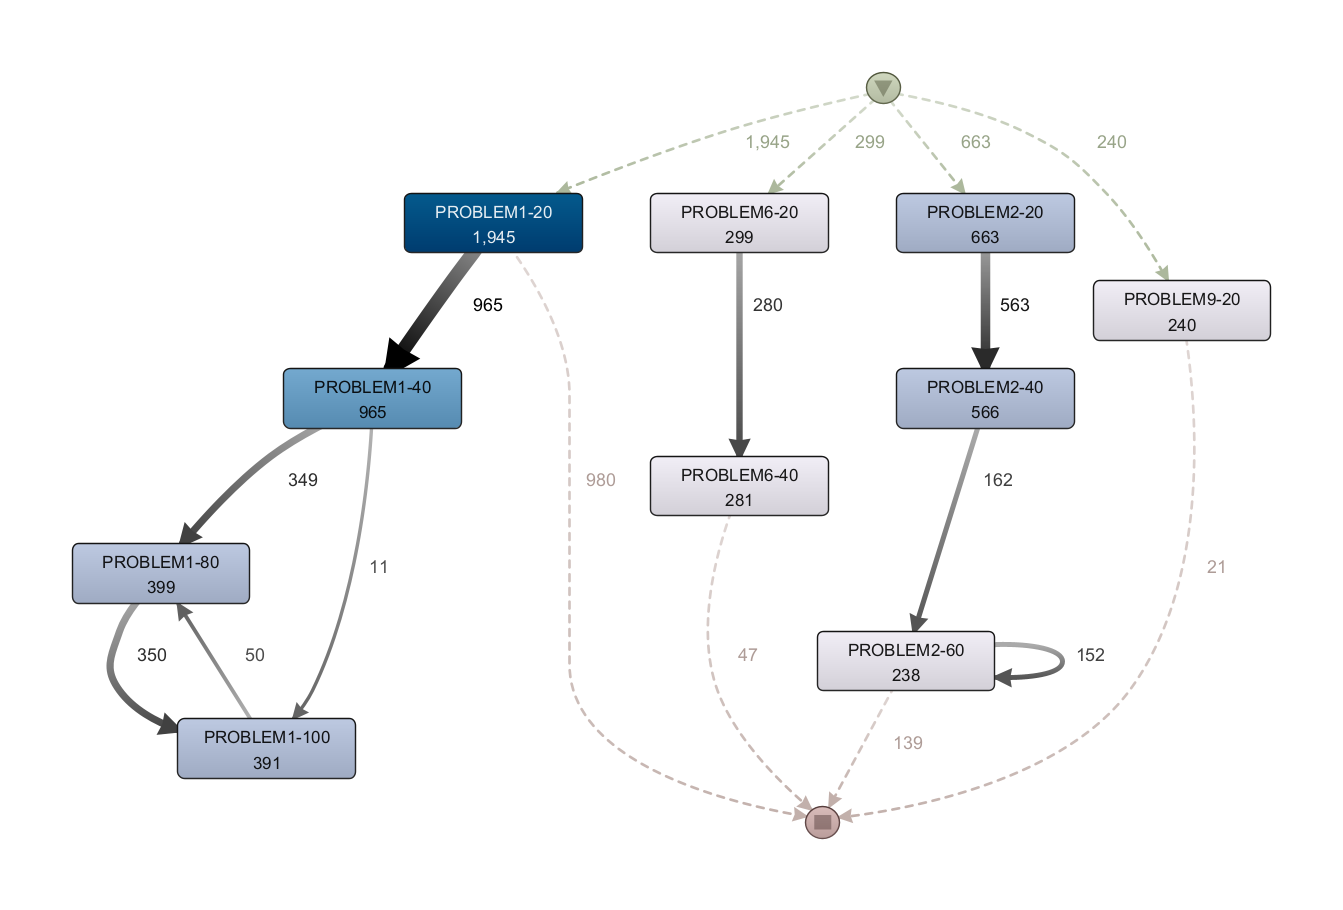
\includegraphics[width=1.25\textwidth]{imagenes/Year1718.png}
    \caption{Extracción de procesos del curso académico 1718.}
    \label{fig:año1718}
\end{figure}

\begin{figure}[H]
    \centering
    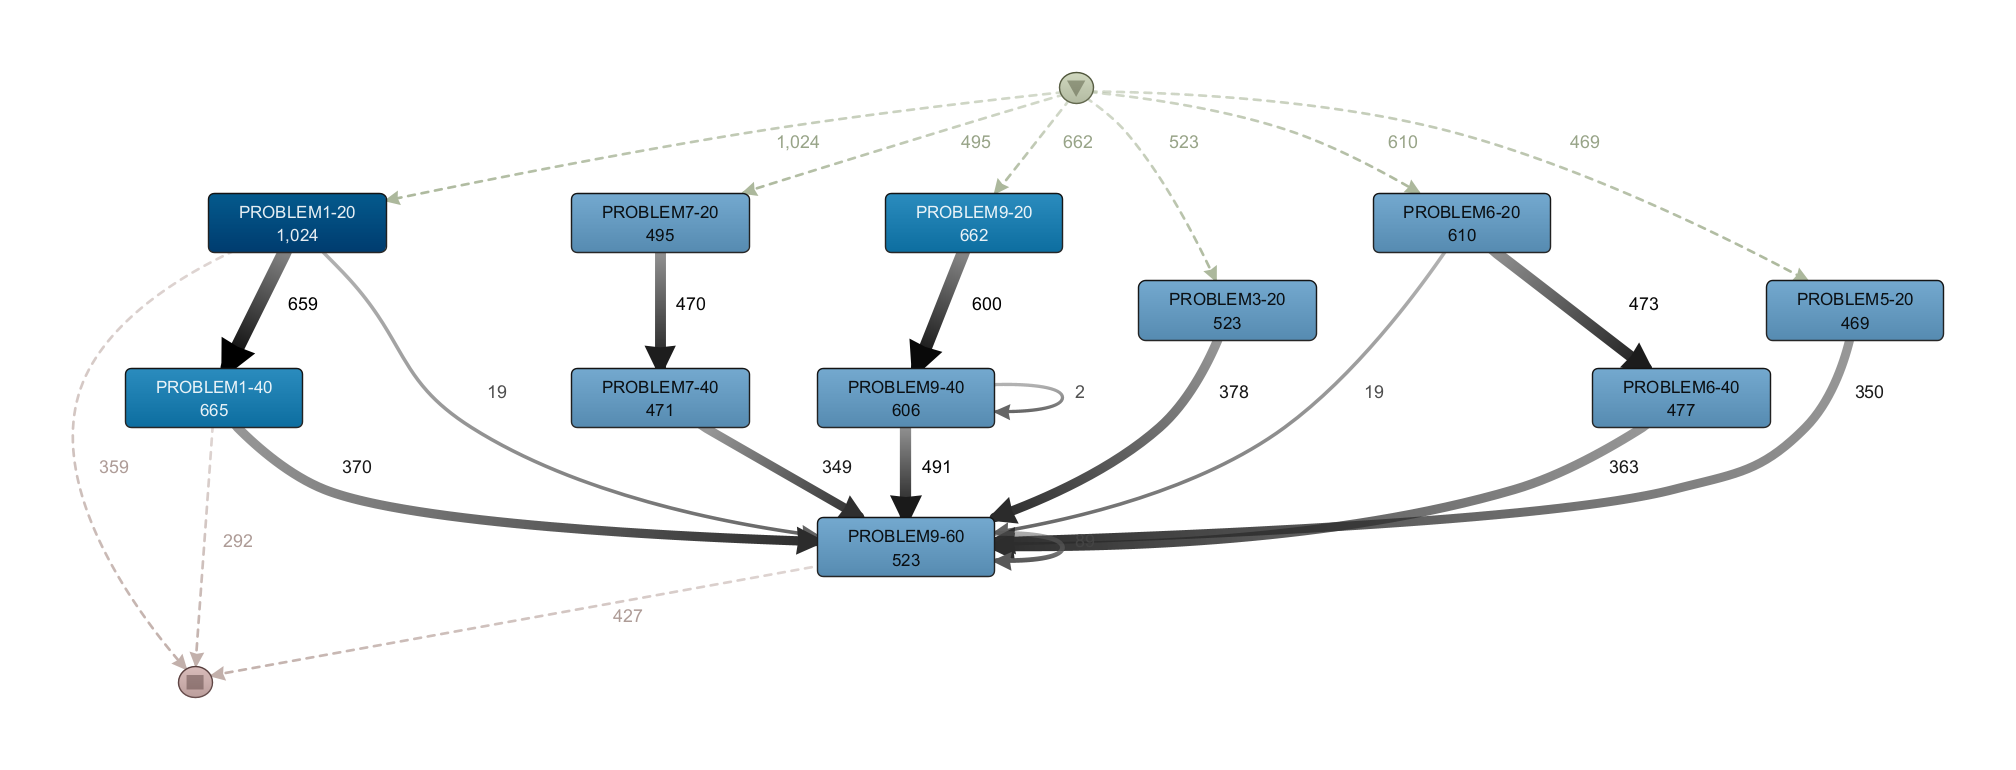
\includegraphics[width=1.25\textwidth]{imagenes/Year1920.png}
    \caption{Extracción de procesos del curso académico 1920.}
    \label{fig:año1920}
\end{figure}

\subsection{Segmentación por calificaciones}

De ahora en adelante se considerará que la calificación de un grupo es \emph{``baja''} si es inferior a $7.5$, \emph{``media-baja''} si es igual o mayor que $7.5$ y menor a $8.5$, \emph{``media-alta''} si es igual a o mayor que $8.5$ e inferior a $9.5$ y \emph{``alta''} si es igual o superior a $9.5$.

\begin{figure}[H]
    \centering
    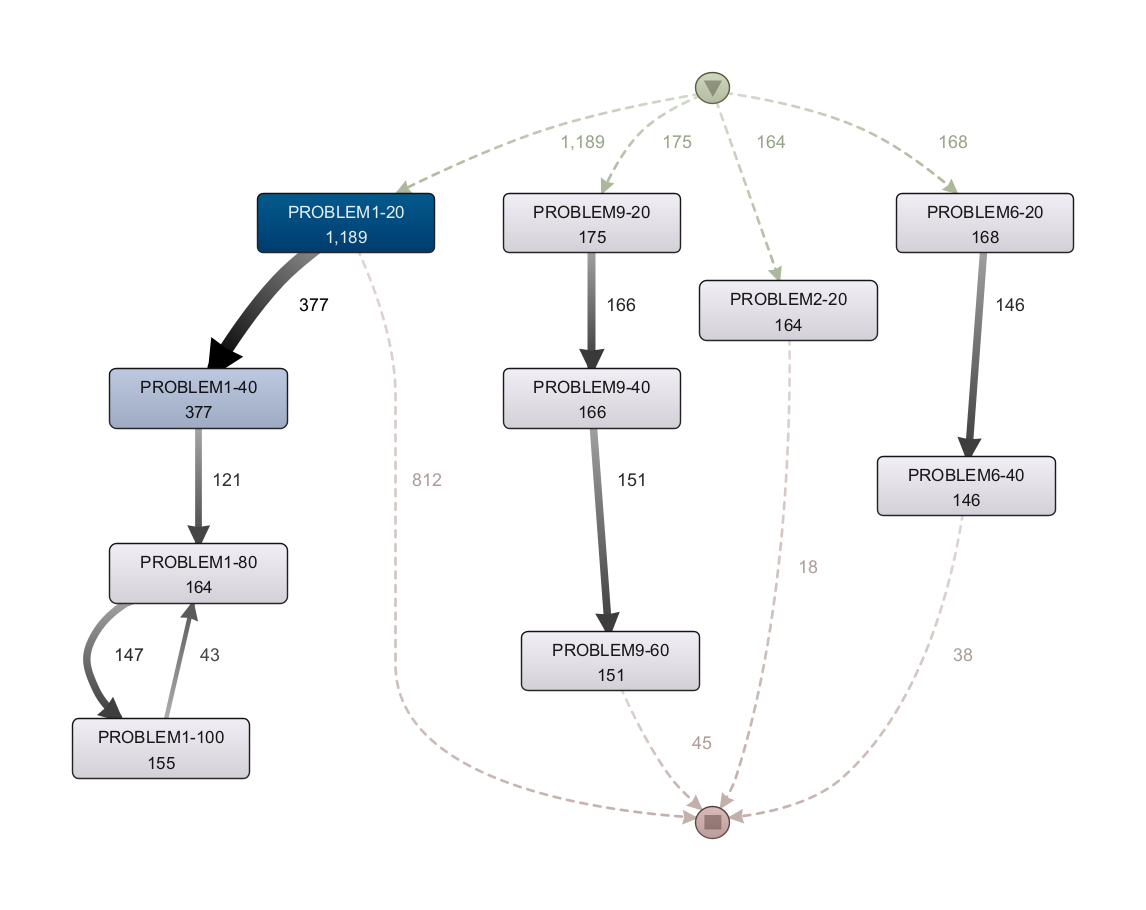
\includegraphics[width=1.25\textwidth]{imagenes/WorstGrades.png}
    \caption{Extracción de procesos del dataset integrado por las acciones compuestas de alumnos con calificación \emph{``baja''}.}
    \label{fig:worstGrades}
\end{figure}

\begin{figure}[H]
    \centering
    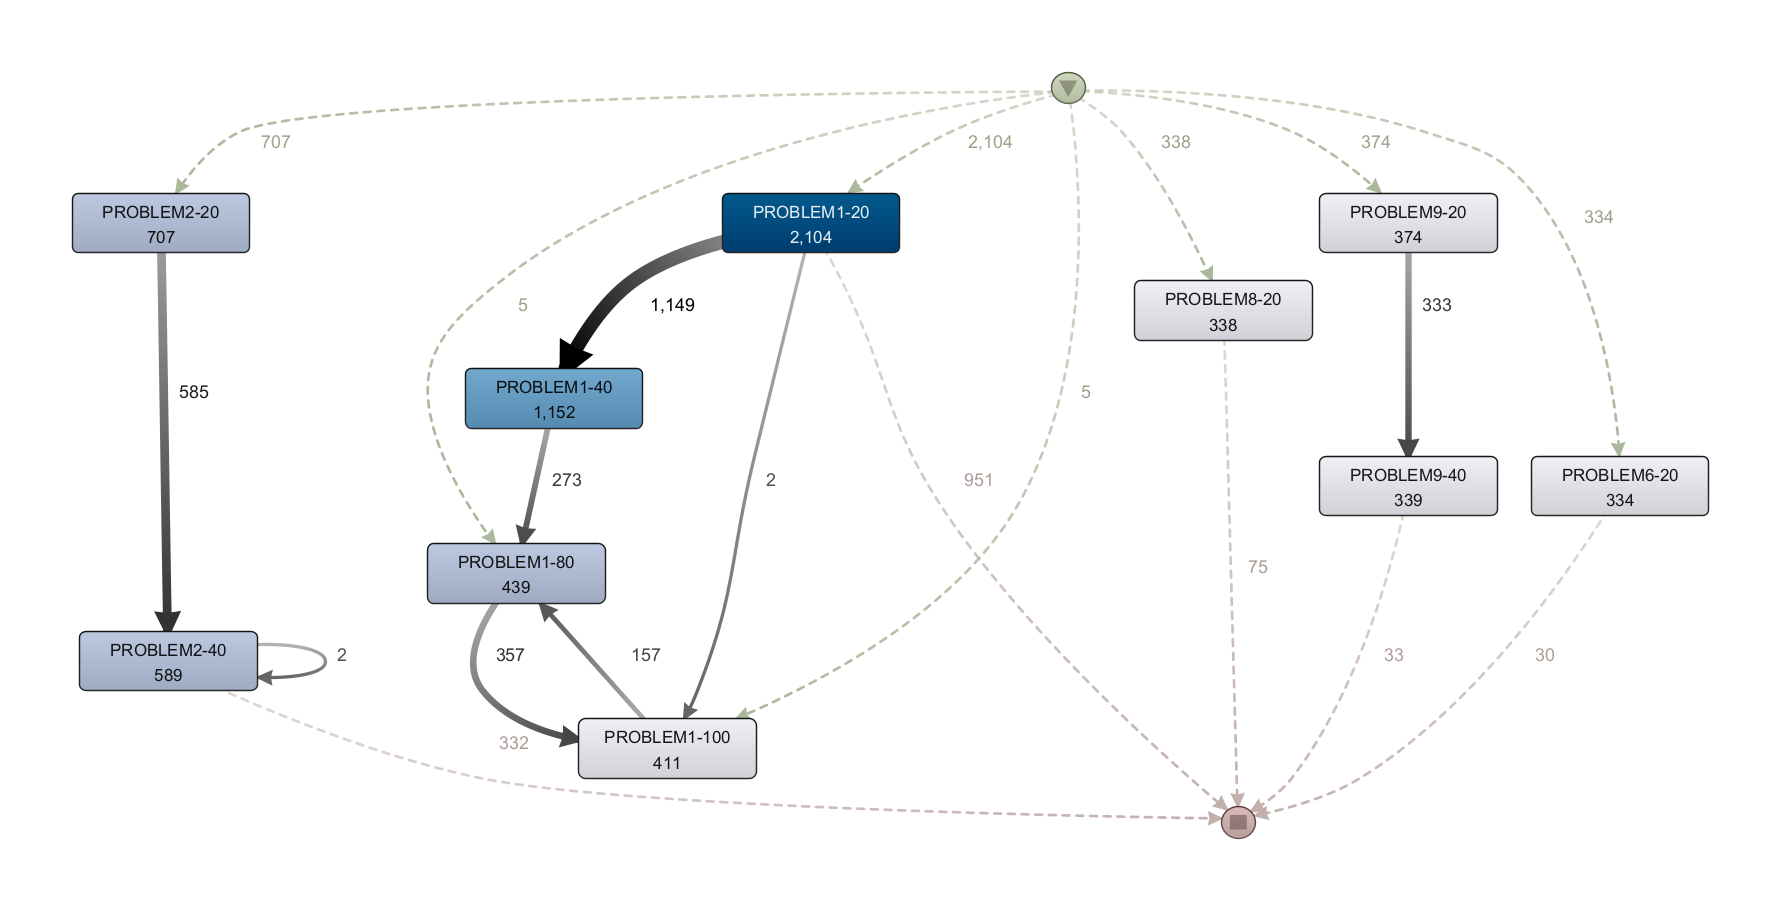
\includegraphics[width=1.25\textwidth]{imagenes/MidLowGrades.png}
    \caption{Extracción de procesos del dataset integrado por las acciones compuestas de alumnos con calificación \emph{``media-baja''}.}
    \label{fig:midLowGrades}
\end{figure}

\begin{figure}[H]
    \centering
    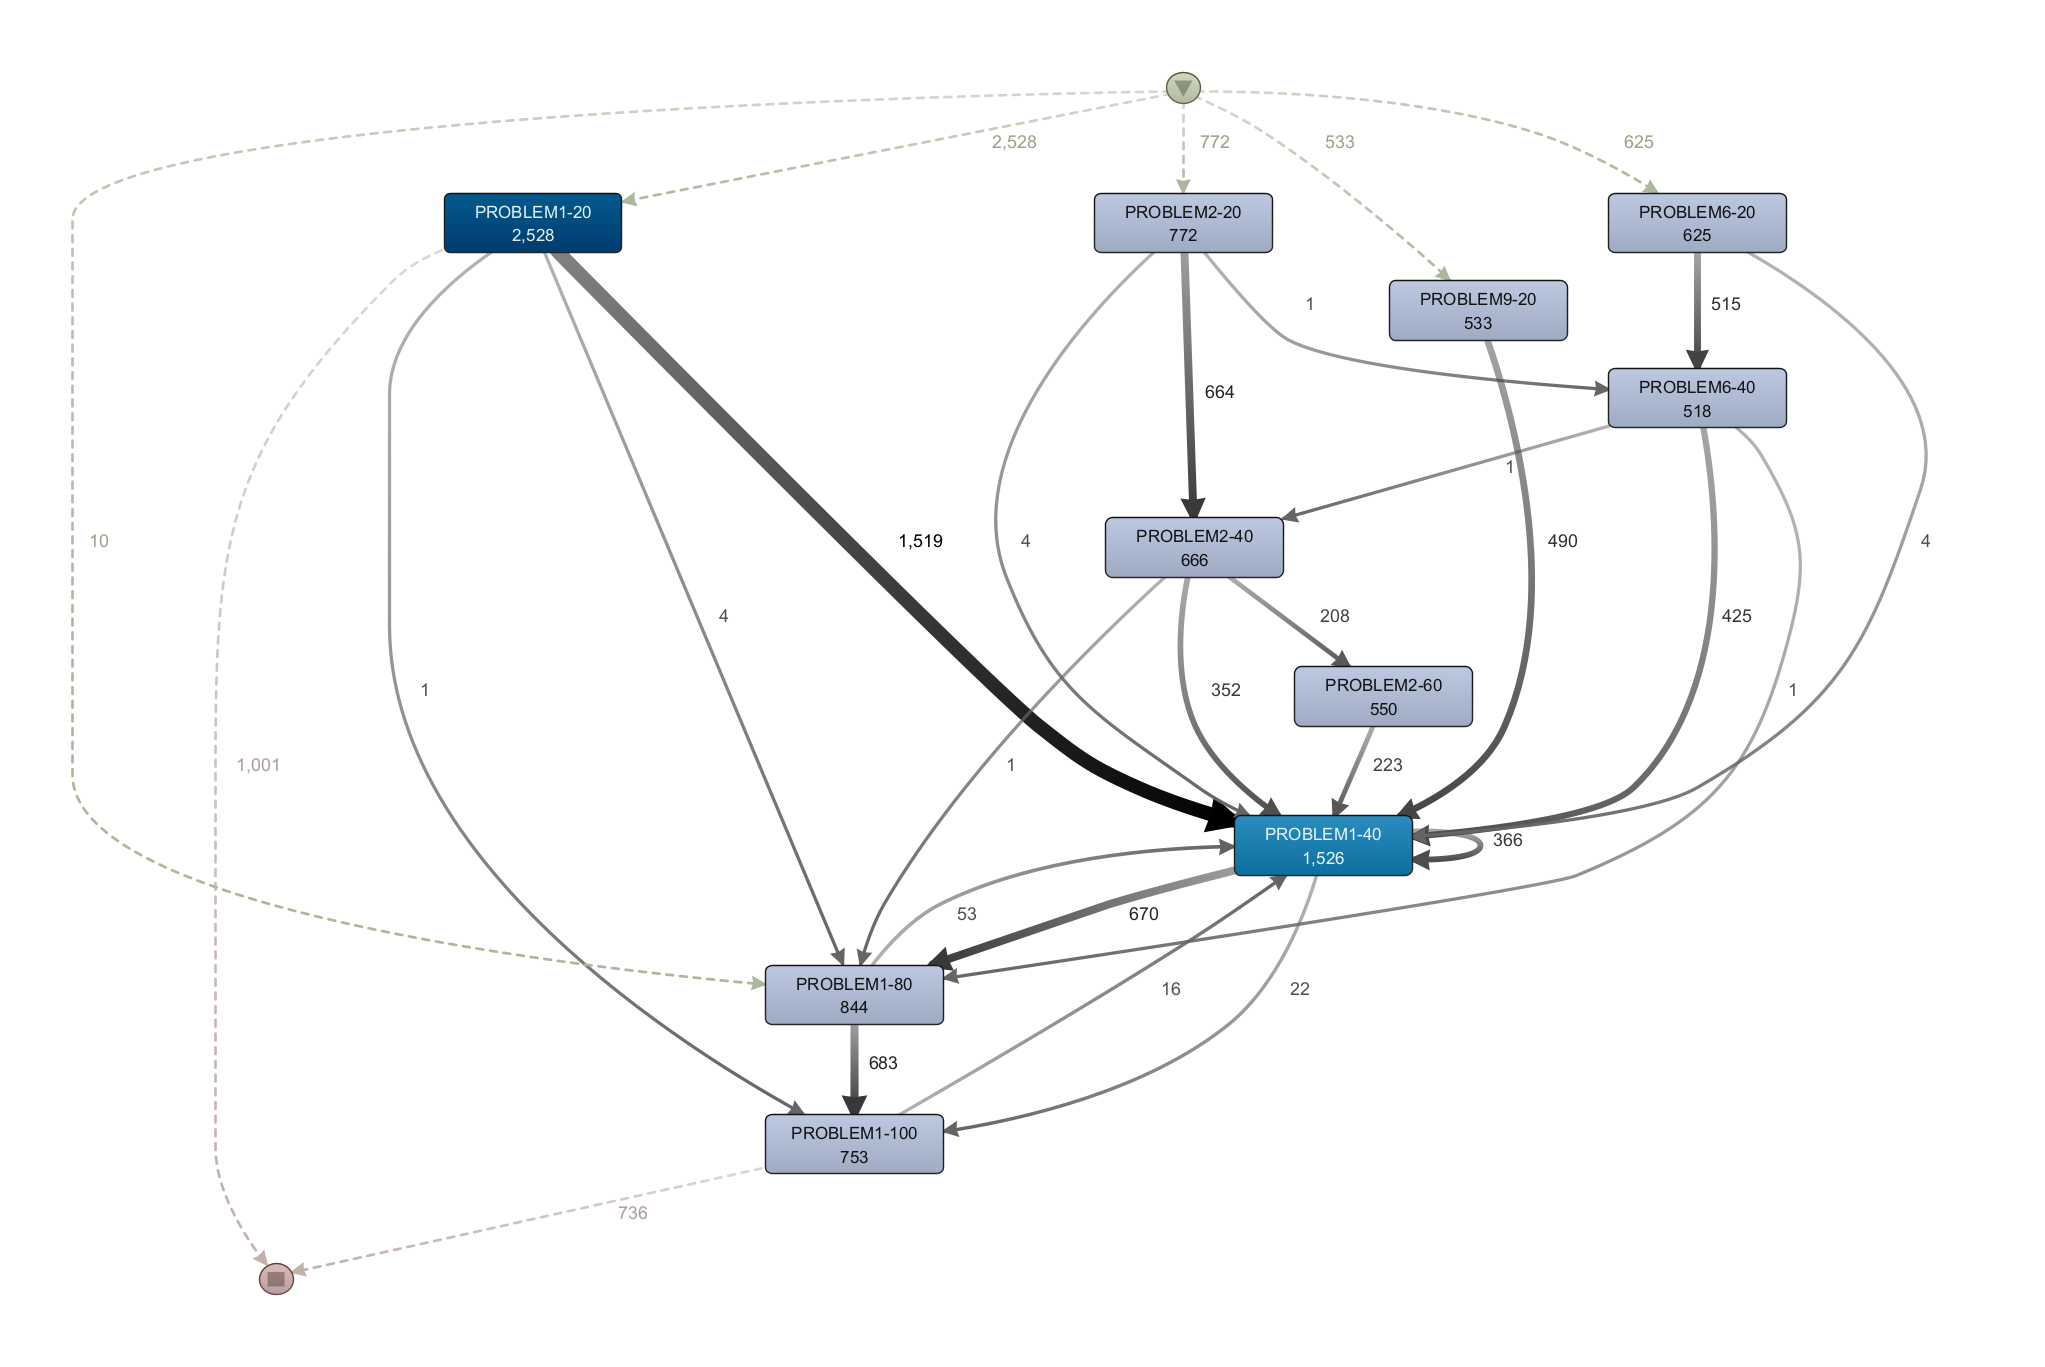
\includegraphics[width=1.25\textwidth]{imagenes/MidHighGrades.png}
    \caption{Extracción de procesos del dataset integrado por las acciones compuestas de alumnos con calificación \emph{``media-alta''}.}
    \label{fig:midHighGrades}
\end{figure}

\begin{figure}[H]
    \centering
    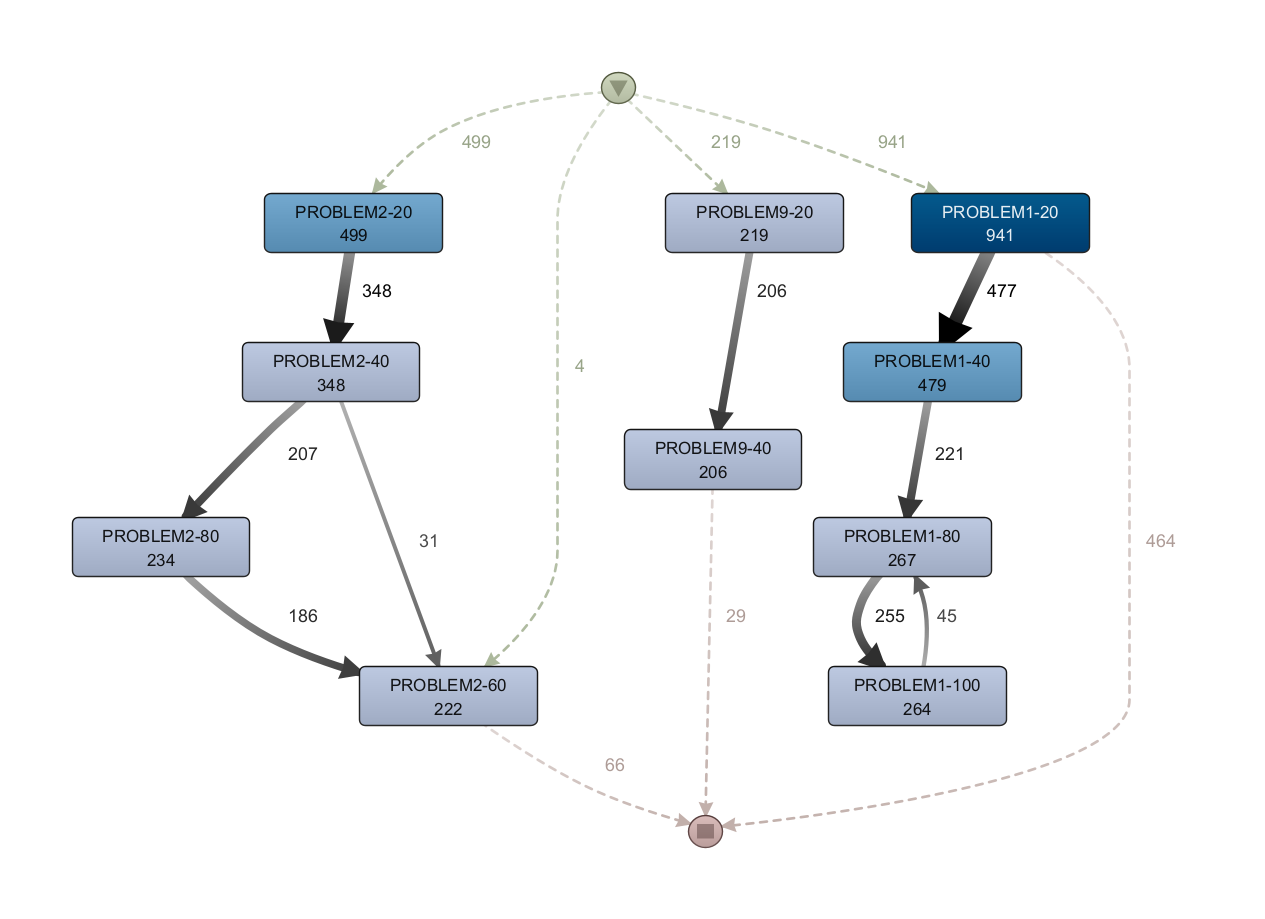
\includegraphics[width=1.25\textwidth]{imagenes/BestGrades.png}
    \caption{Extracción de procesos del dataset integrado por las acciones compuestas de alumnos con calificación \emph{``alta''}.}
    \label{fig:bestGrades}
\end{figure}


\subsection{Segmentación por año y calificación}

\begin{figure}[H]
    \centering
    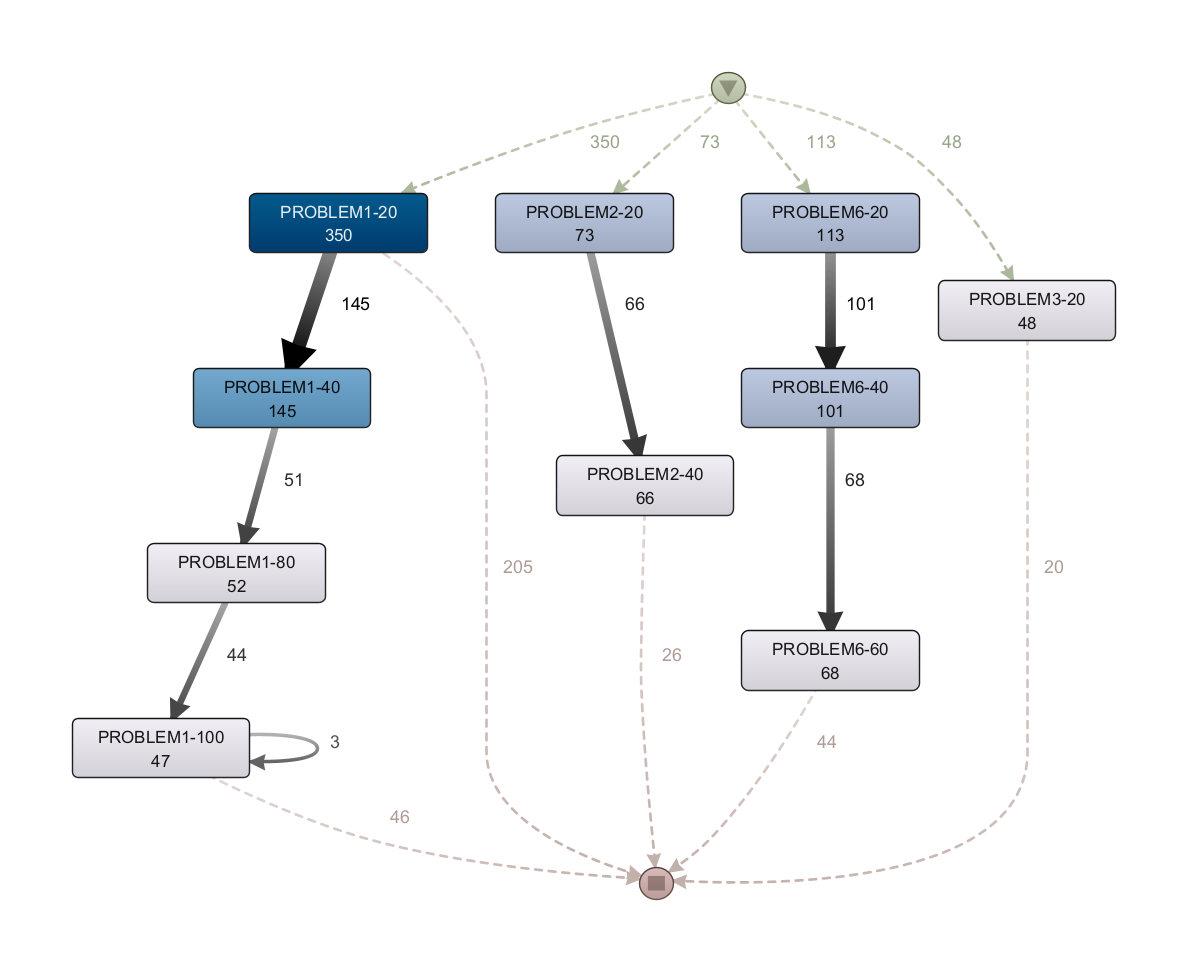
\includegraphics[width=1.25\textwidth]{imagenes/Year1617WorstGrades.png}
    \caption{Extracción de procesos del dataset integrado por las acciones compuestas de alumnos con calificación \emph{``baja''} del curso académico 1617.}
    \label{fig:year1617WorstGrades}
\end{figure}

\begin{figure}[H]
    \centering
    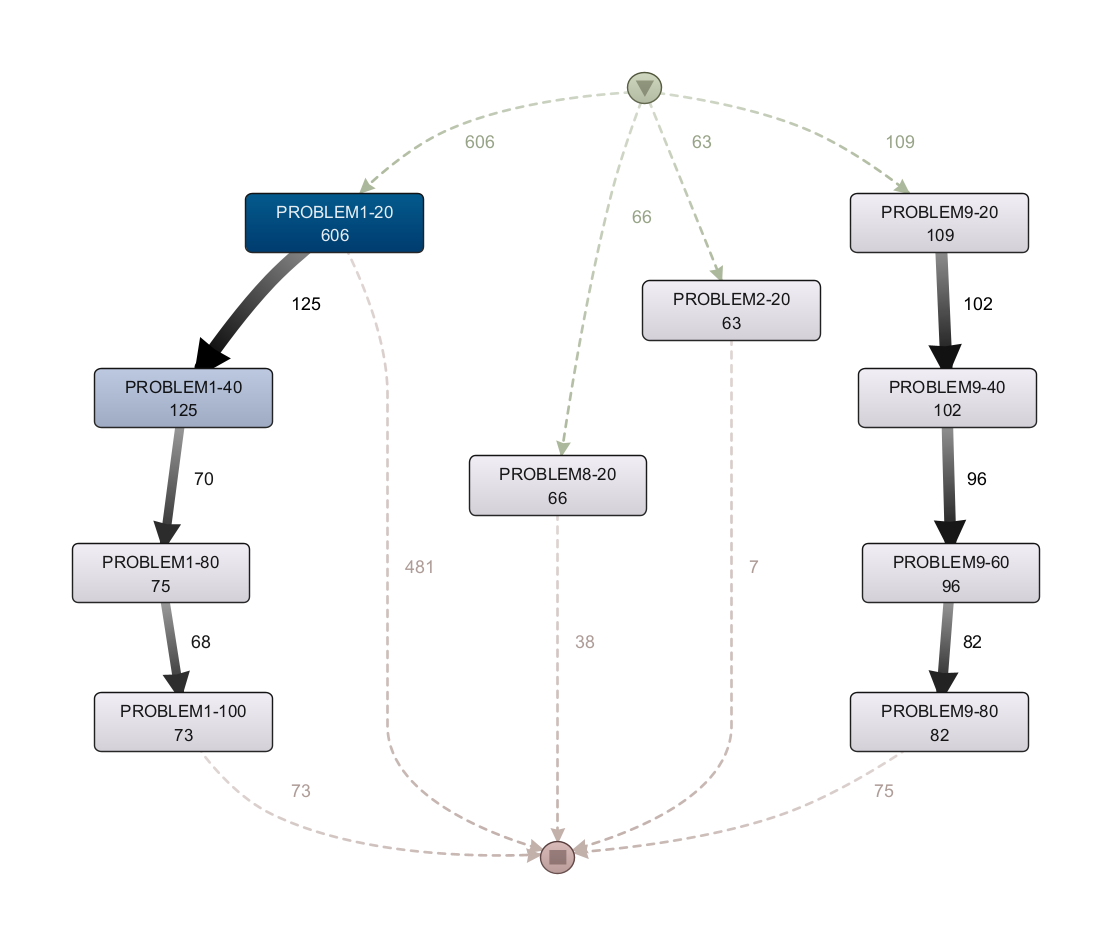
\includegraphics[width=1.25\textwidth]{imagenes/Year1718WorstGrades.png}
    \caption{Extracción de procesos del dataset integrado por las acciones compuestas de alumnos con calificación \emph{``baja''} del curso académico 1718.}
    \label{fig:year1718WorstGrades}
\end{figure}

\begin{figure}[H]
    \centering
    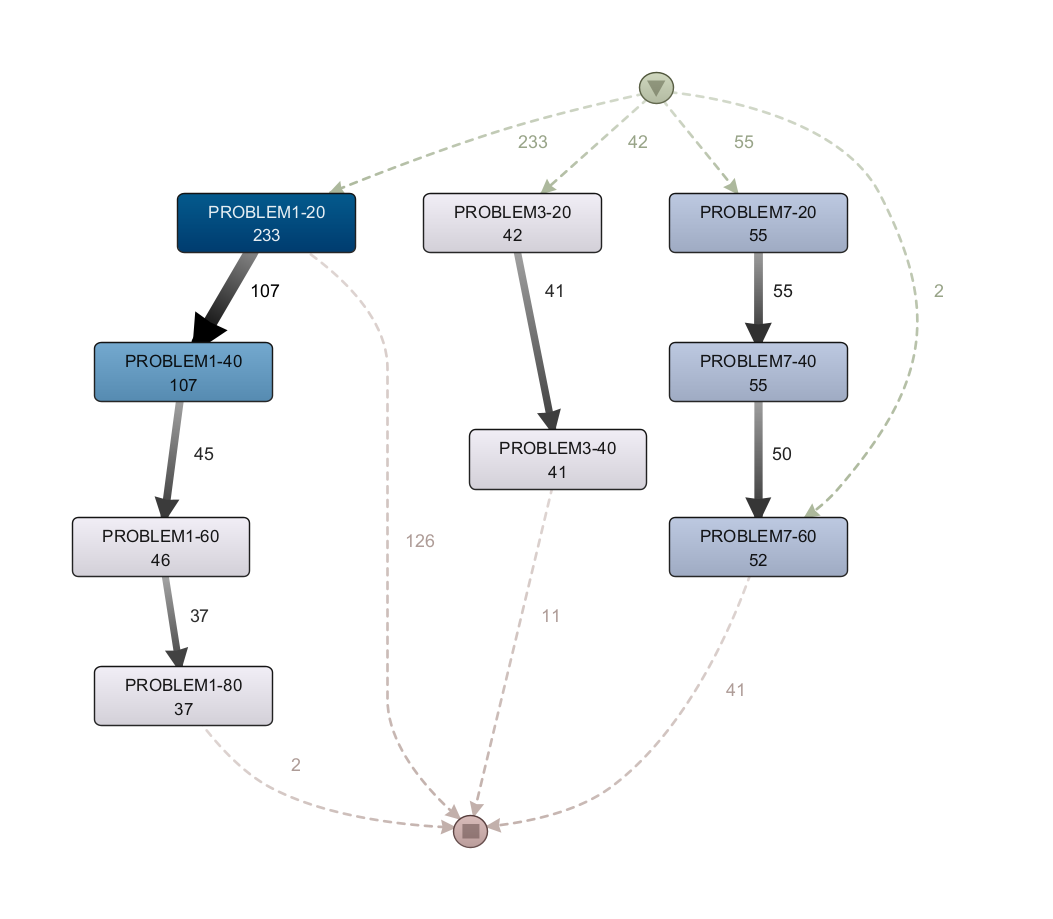
\includegraphics[width=1.25\textwidth]{imagenes/Year1920WorstGrades.png}
    \caption{Extracción de procesos del dataset integrado por las acciones compuestas de alumnos con calificación \emph{``baja''} del curso académico 1920.}
    \label{fig:year1920WorstGrades}
\end{figure}

\begin{figure}[H]
    \centering
    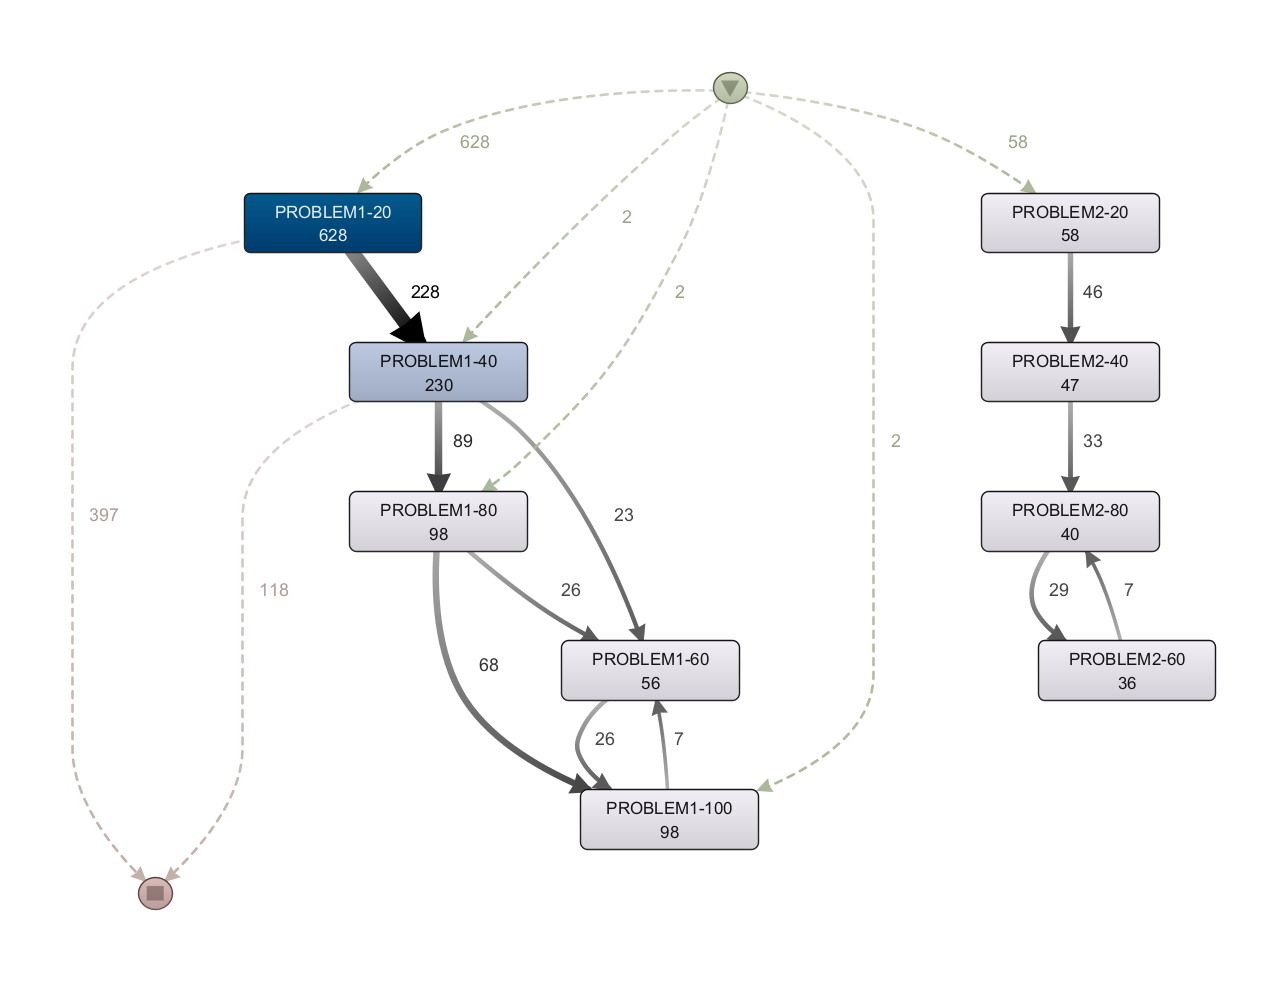
\includegraphics[width=1.25\textwidth]{imagenes/Year1516MidLowGrades.png}
    \caption{Extracción de procesos del dataset integrado por las acciones compuestas de alumnos con calificación \emph{``media-baja''} del curso académico 1516.}
    \label{fig:year1516MidLowGrades}
\end{figure}

\begin{figure}[H]
    \centering
    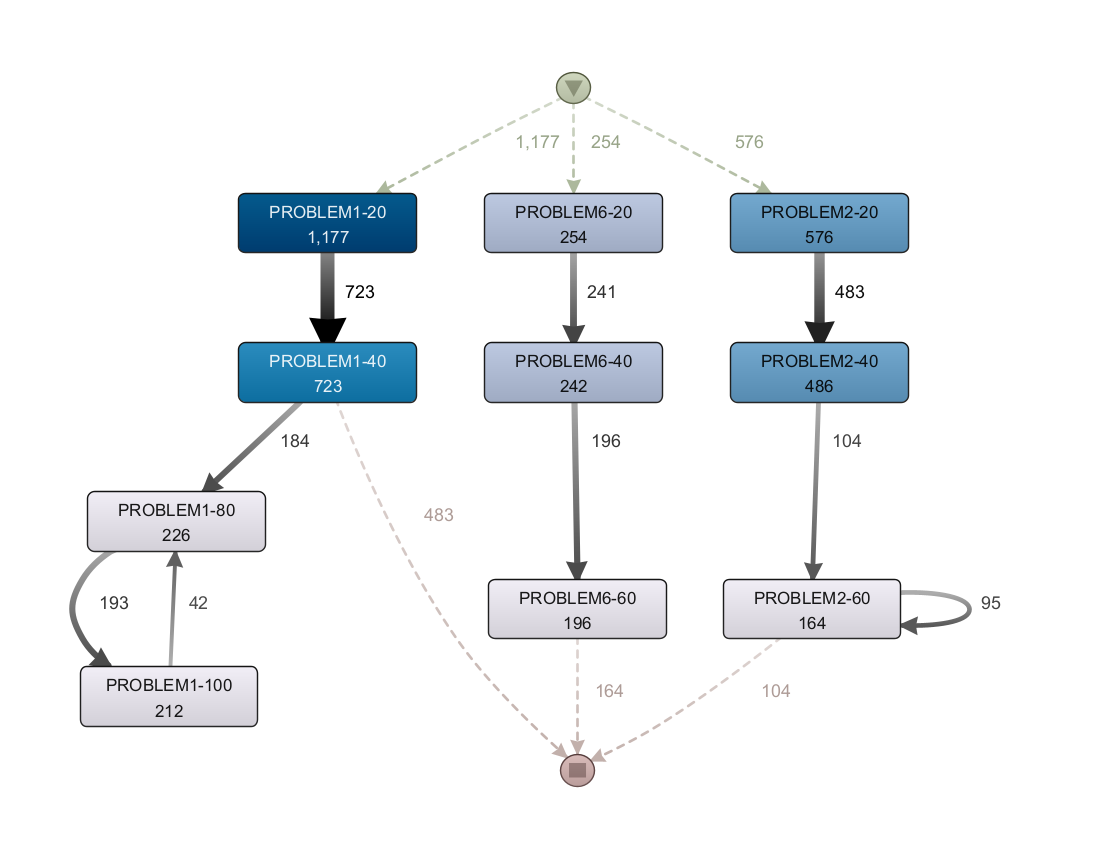
\includegraphics[width=1.25\textwidth]{imagenes/Year1718MidLowGrades.png}
    \caption{Extracción de procesos del dataset integrado por las acciones compuestas de alumnos con calificación \emph{``media-baja''} del curso académico 1718.}
    \label{fig:year1718MidLowGrades}
\end{figure}

\begin{figure}[H]
    \centering
    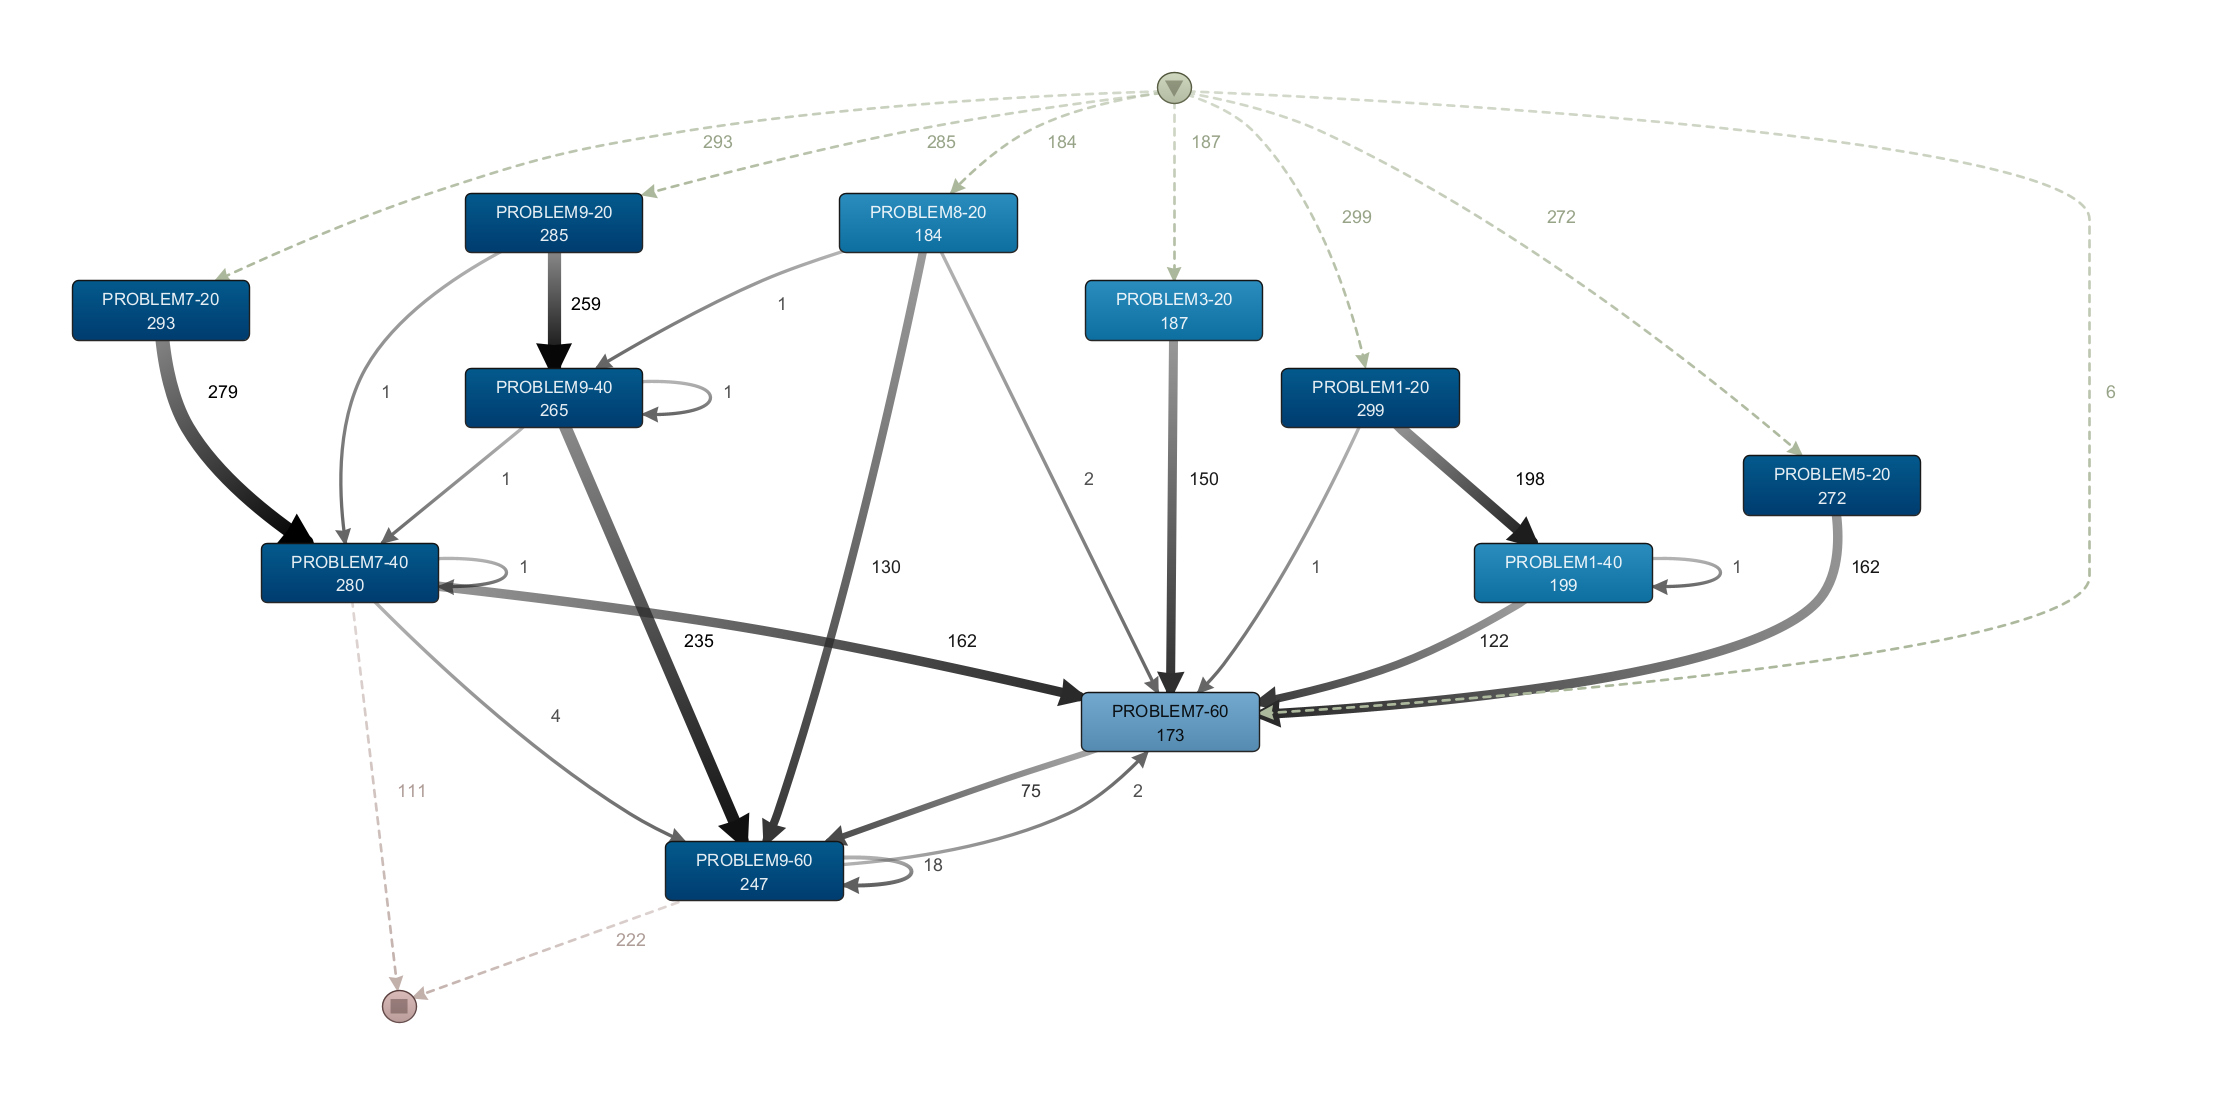
\includegraphics[width=1.25\textwidth]{imagenes/Year1920MidLowGrades.png}
    \caption{Extracción de procesos del dataset integrado por las acciones compuestas de alumnos con calificación \emph{``media-baja''} del curso académico 1920.}
    \label{fig:year1920MidLowGrades}
\end{figure}

\begin{figure}[H]
    \centering
    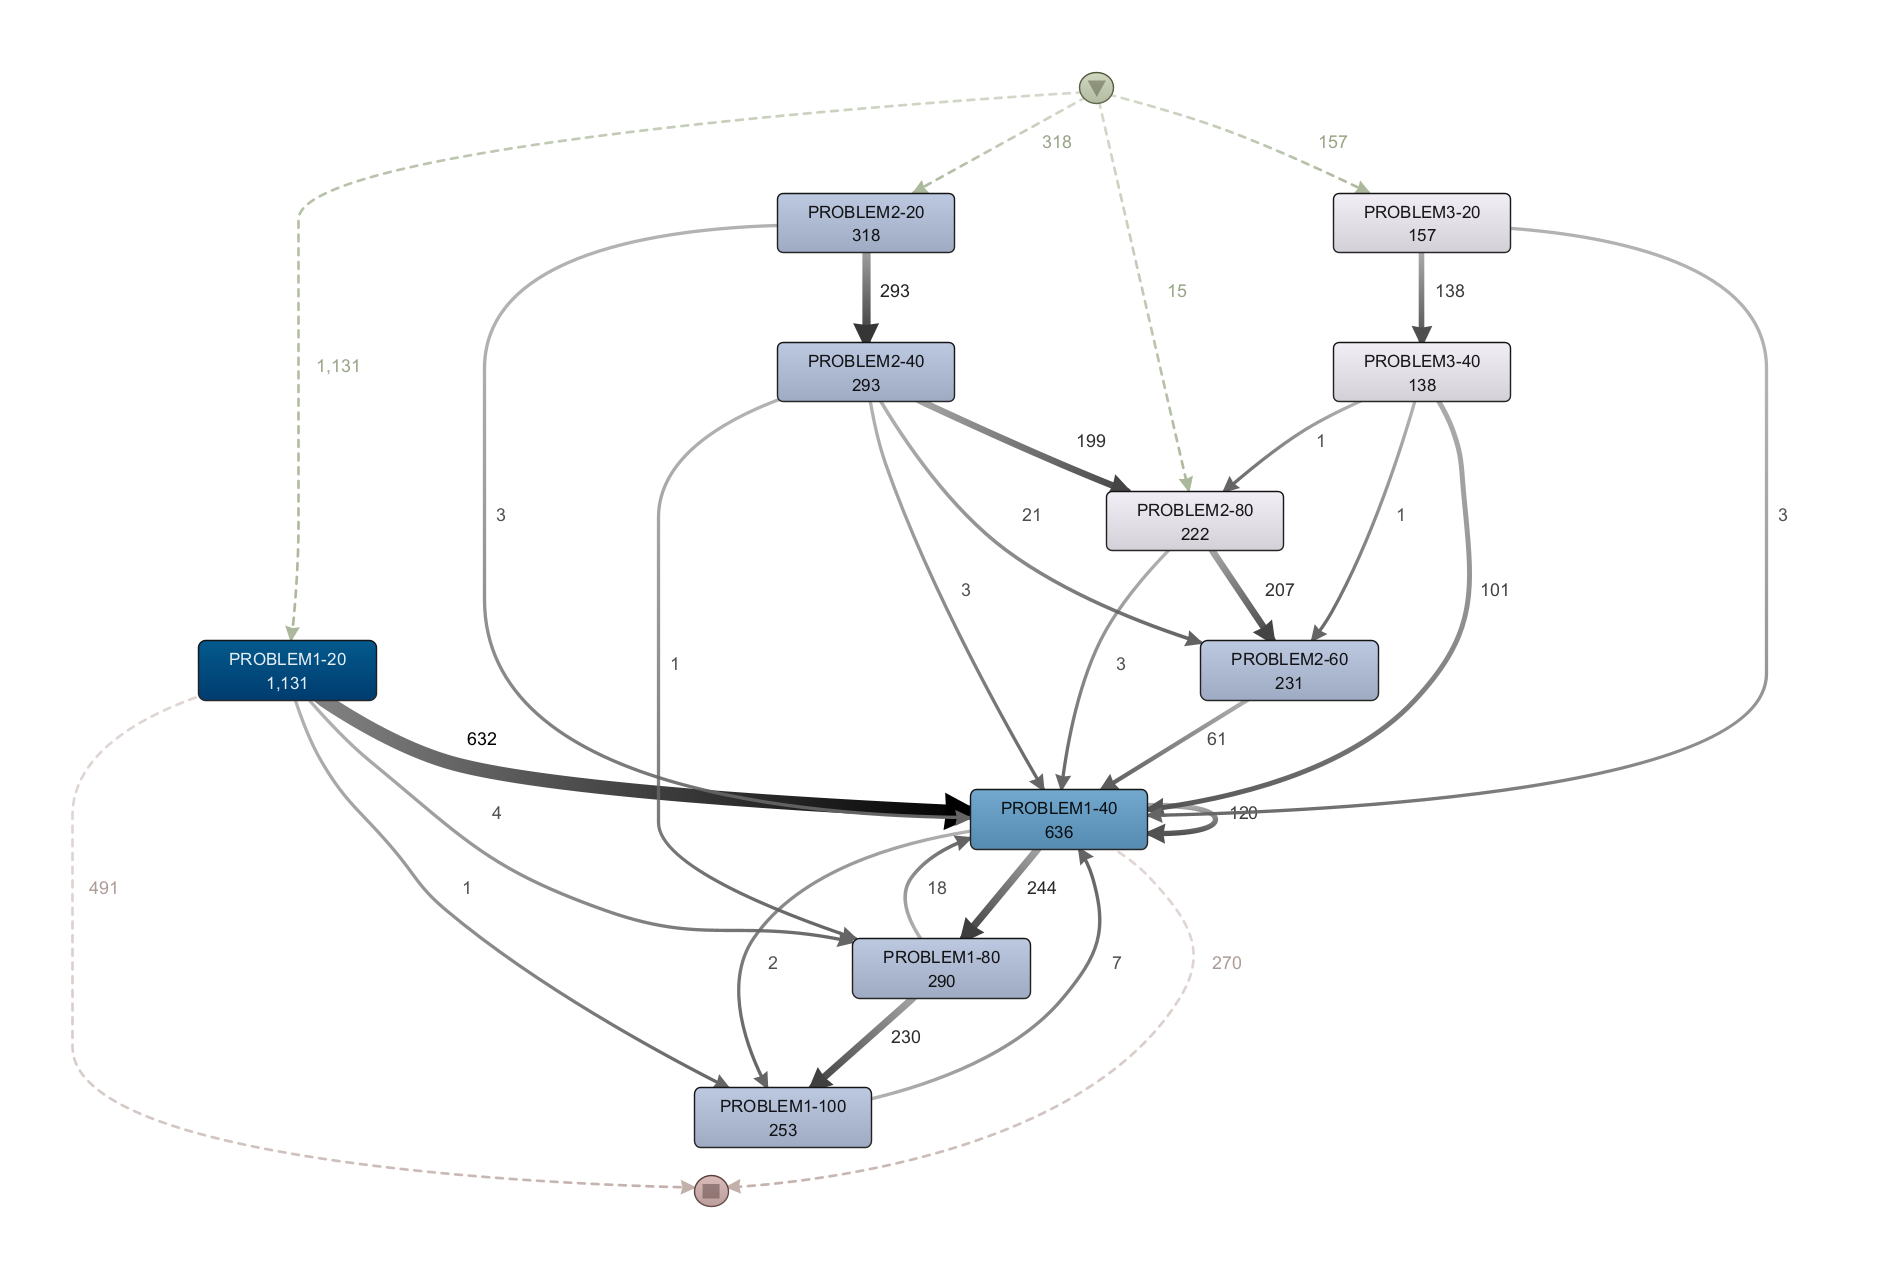
\includegraphics[width=1.25\textwidth]{imagenes/Year1516MidHighGrades.png}
    \caption{Extracción de procesos del dataset integrado por las acciones compuestas de alumnos con calificación \emph{``media-alta''} del curso académico 1516.}
    \label{fig:year1516MidHighGrades}
\end{figure}

\begin{figure}[H]
    \centering
    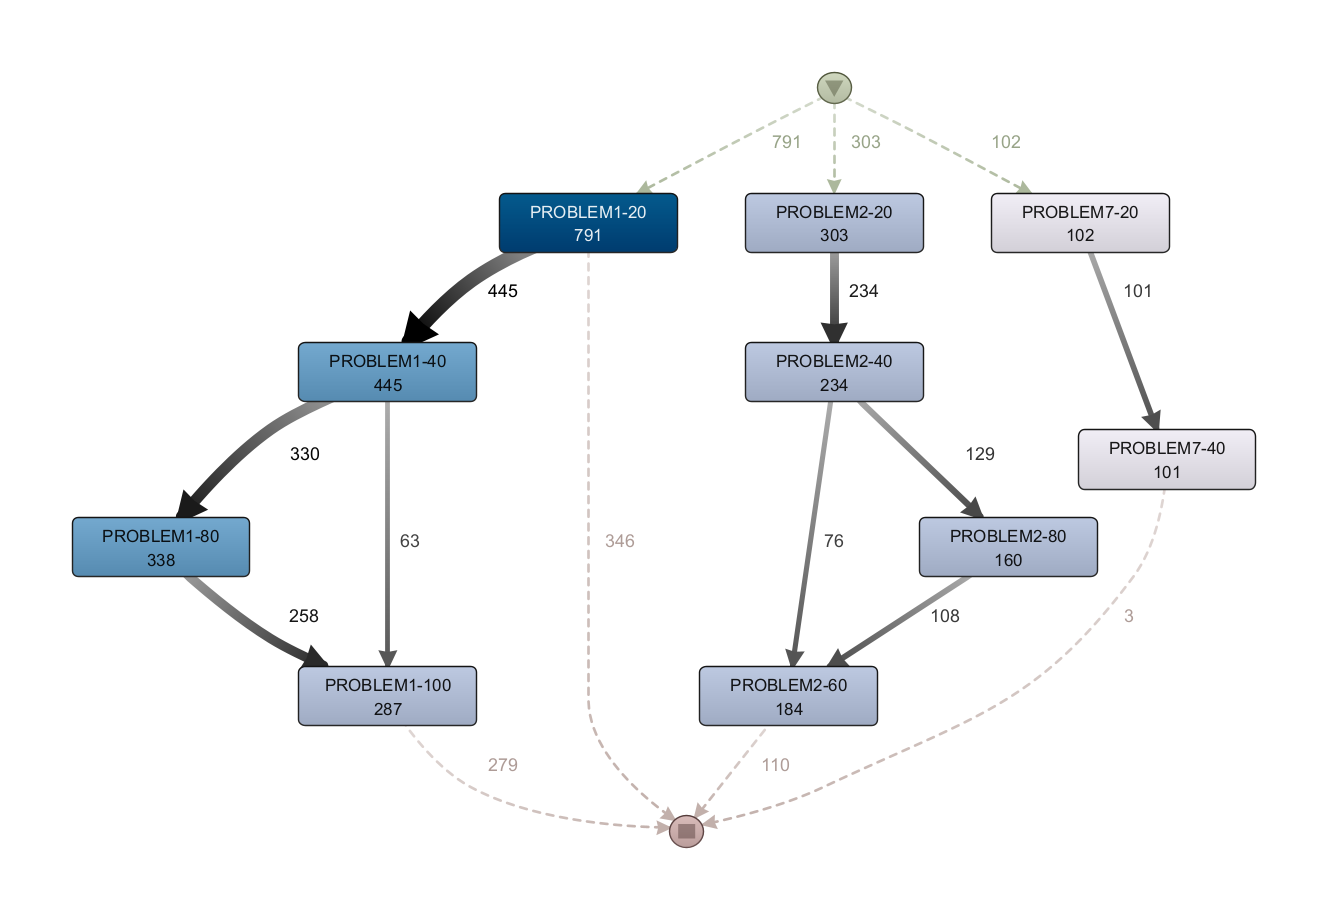
\includegraphics[width=1.25\textwidth]{imagenes/Year1617MidHighGrades.png}
    \caption{Extracción de procesos del dataset integrado por las acciones compuestas de alumnos con calificación \emph{``media-alta''} del curso académico 1617.}
    \label{fig:year1617MidHighGrades}
\end{figure}

\begin{figure}[H]
    \centering
    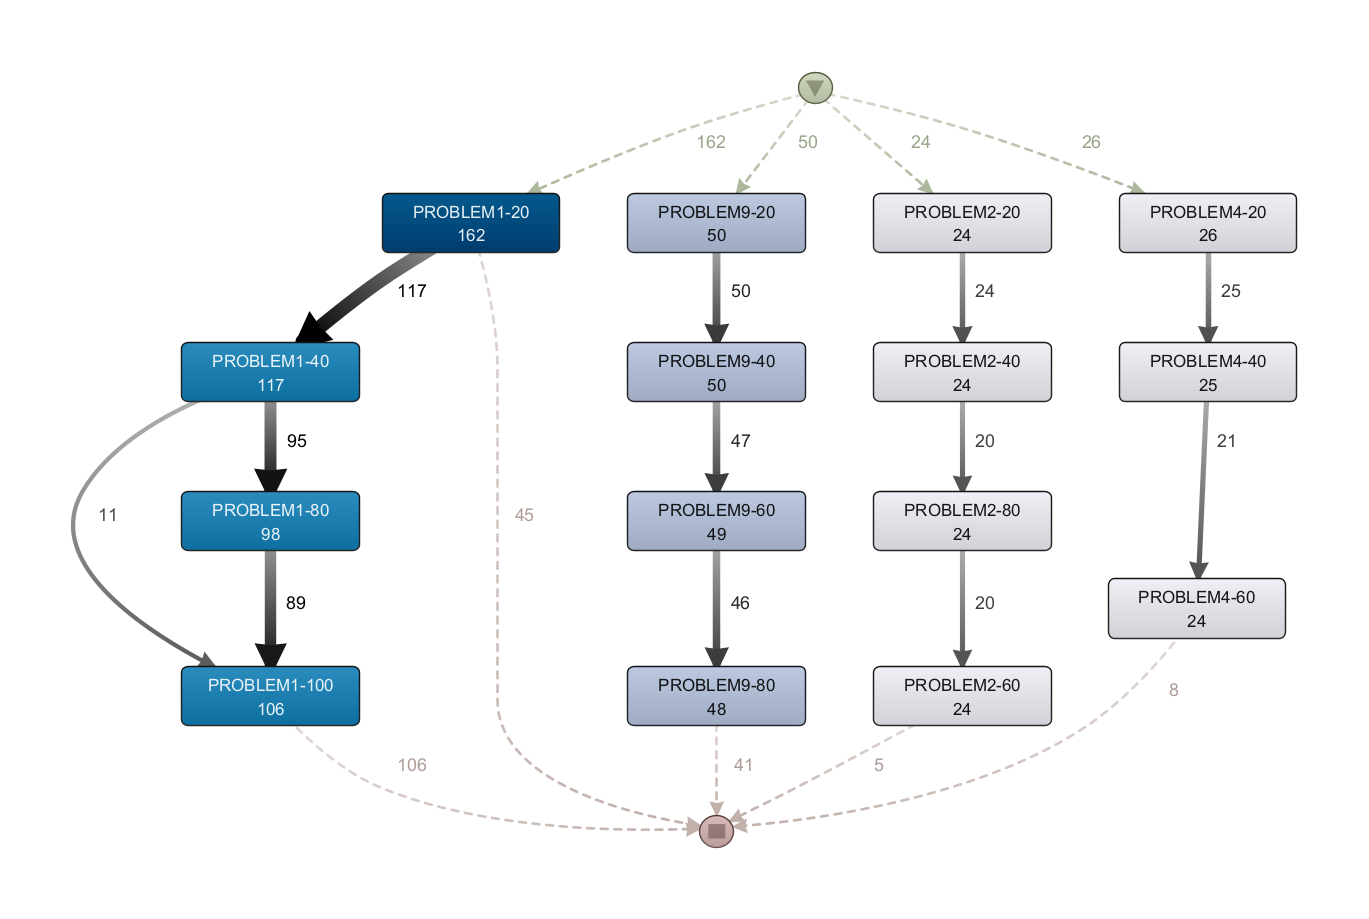
\includegraphics[width=1.25\textwidth]{imagenes/Year1718MidHighGrades.png}
    \caption{Extracción de procesos del dataset integrado por las acciones compuestas de alumnos con calificación \emph{``media-alta''} del curso académico 1718.}
    \label{fig:year1718MidHighGrades}
\end{figure}

\begin{figure}[H]
    \centering
    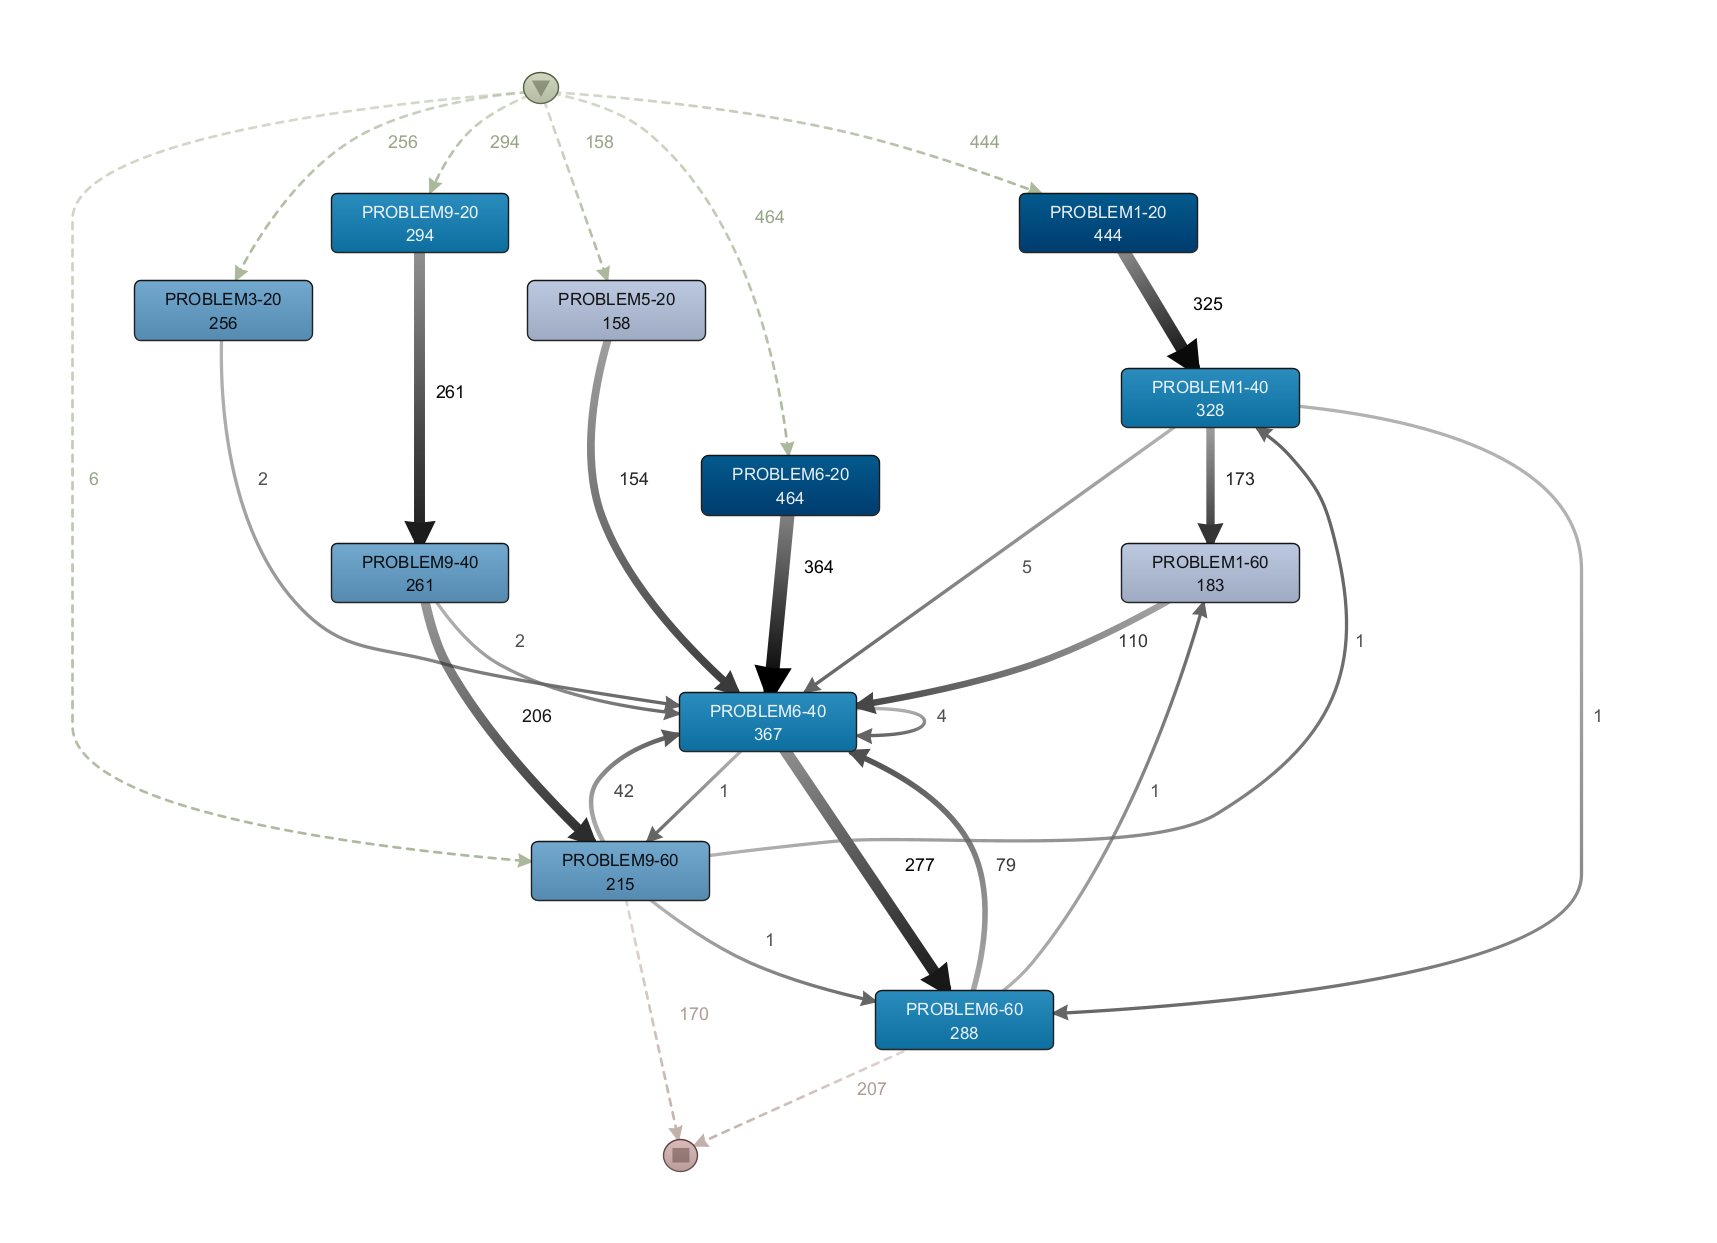
\includegraphics[width=1.25\textwidth]{imagenes/Year1920MidHighGrades.png}
    \caption{Extracción de procesos del dataset integrado por las acciones compuestas de alumnos con calificación \emph{``media-alta''} del curso académico 1920.}
    \label{fig:year1920MidHighGrades}
\end{figure}

\begin{figure}[H]
    \centering
    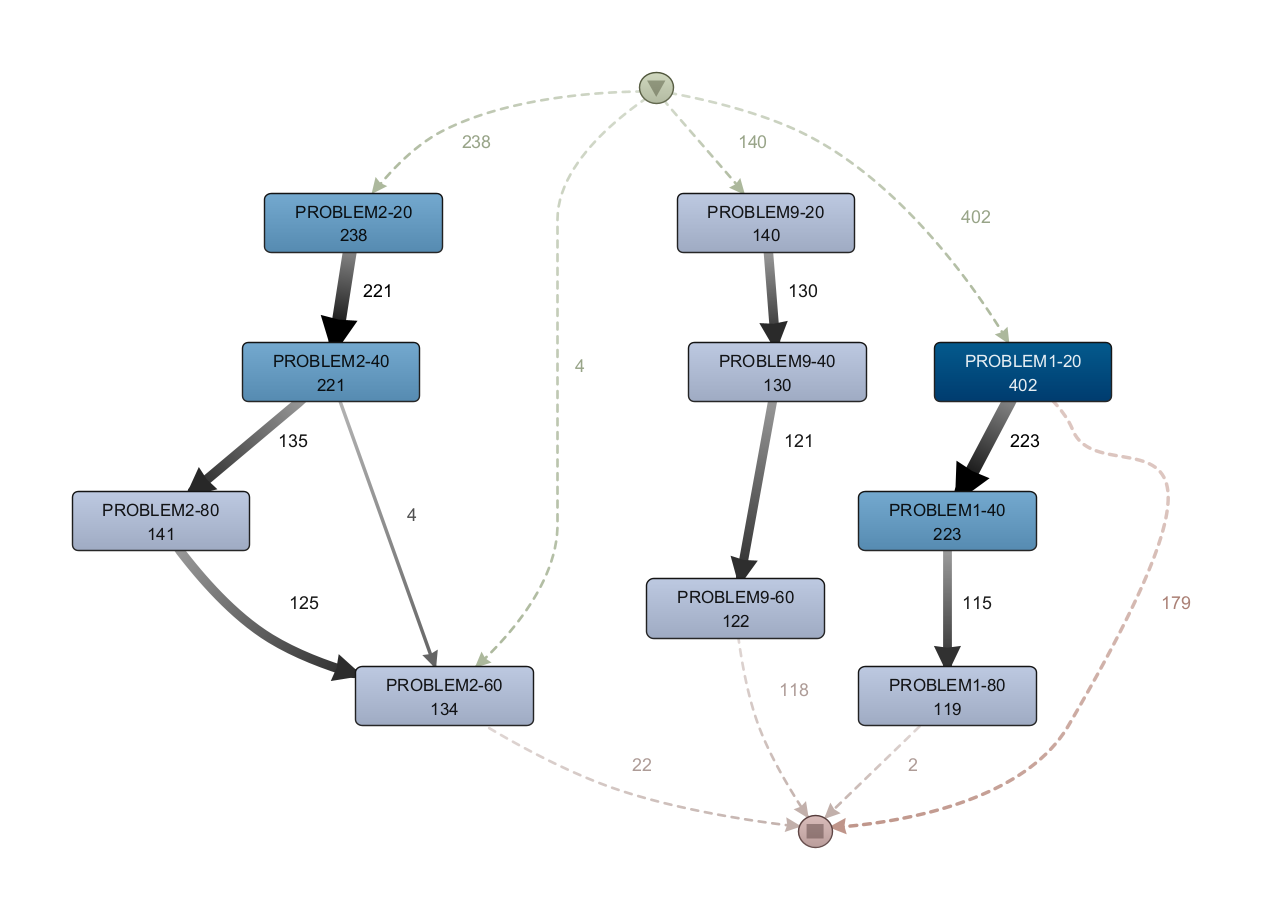
\includegraphics[width=1.25\textwidth]{imagenes/Year1516HighGrades.png}
    \caption{Extracción de procesos del dataset integrado por las acciones compuestas de alumnos con calificación \emph{``alta''} del curso académico 1516.}
    \label{fig:year1516BestGrades}
\end{figure}

\begin{figure}[H]
    \centering
    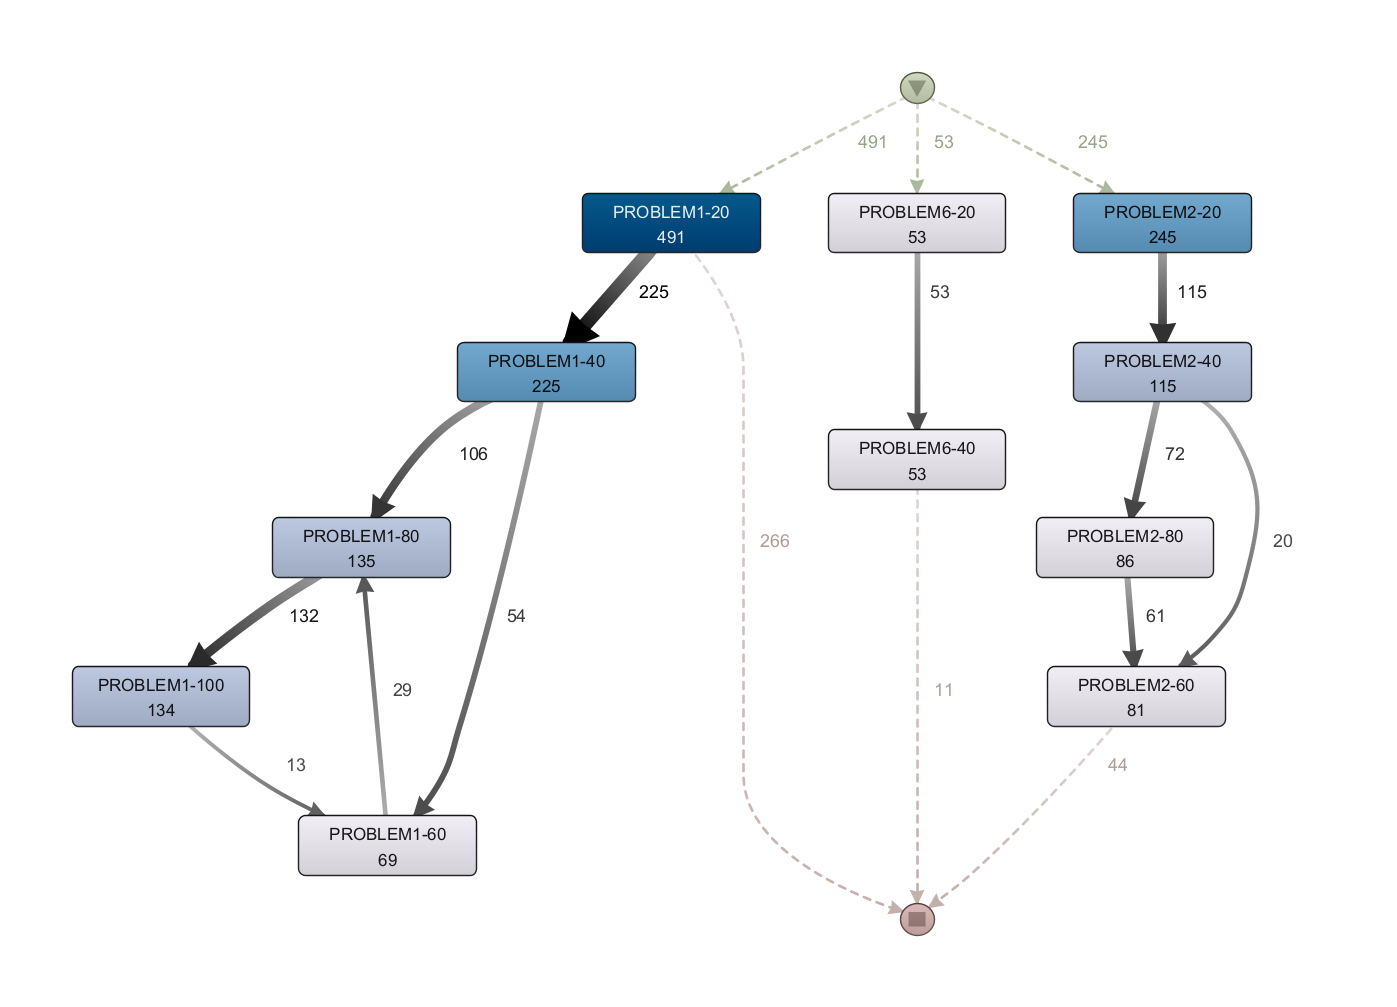
\includegraphics[width=1.25\textwidth]{imagenes/Year1617HighGrades.png}
    \caption{Extracción de procesos del dataset integrado por las acciones compuestas de alumnos con calificación \emph{``alta''} del curso académico 1617.}
    \label{fig:year1617BestGrades}
\end{figure}

\begin{figure}[H]
    \centering
    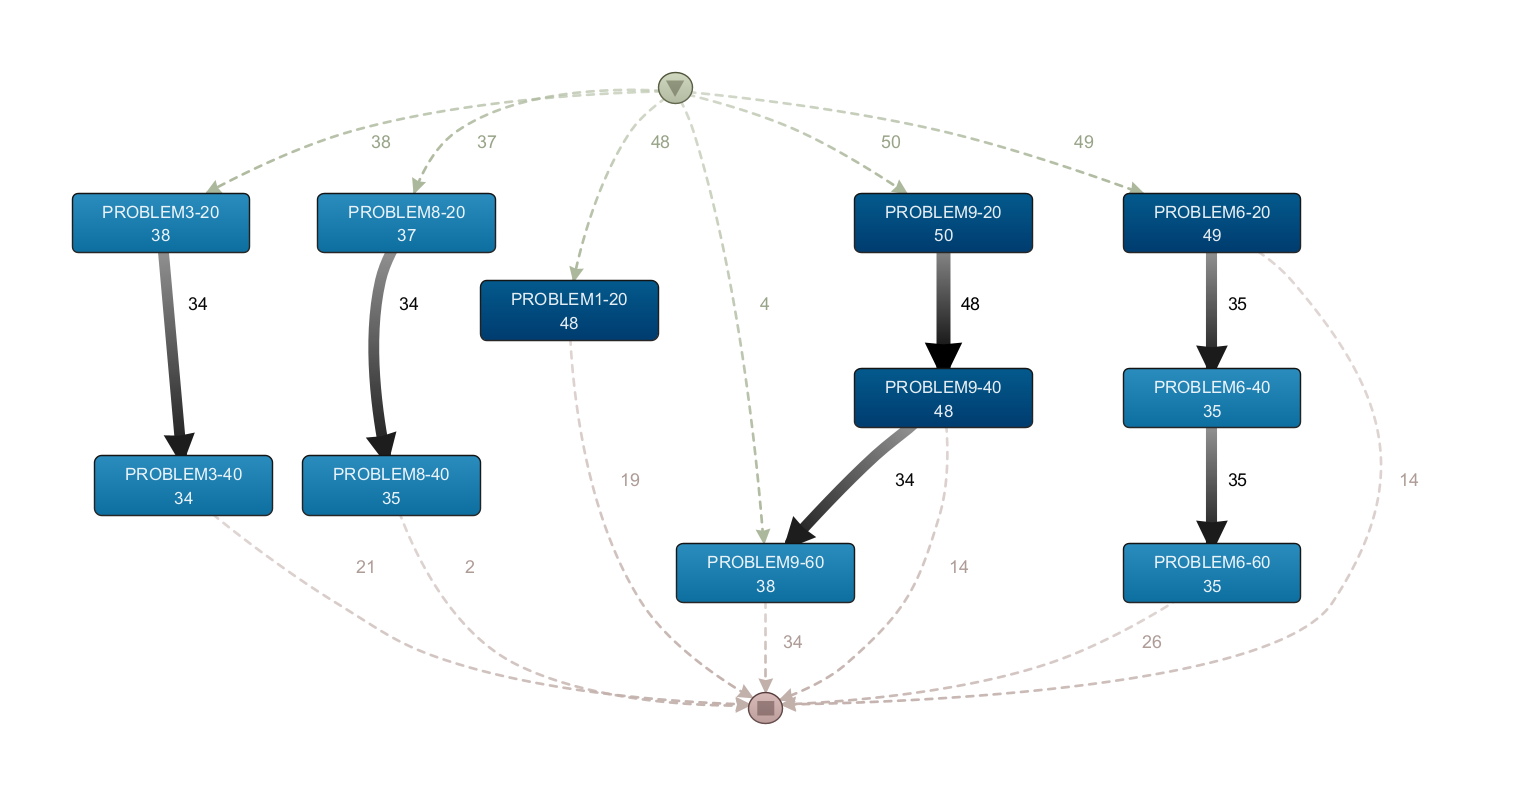
\includegraphics[width=1.25\textwidth]{imagenes/Year1920HighGrades.png}
    \caption{Extracción de procesos del dataset integrado por las acciones compuestas de alumnos con calificación \emph{``alta''} del curso académico 1920.}
    \label{fig:year1920BestGrades}
\end{figure}